\documentclass{article}
\usepackage{amsmath,amssymb}
\DeclareMathOperator{\E}{\mathbb{E}} % For the expectation style E
\usepackage{graphicx}
\usepackage{tabularx}
\usepackage[a4paper, total={6.5in, 10in}]{geometry} % Set margin size.
%\usepackage{subfigure}
\usepackage{subcaption}

\usepackage{amsfonts}
\usepackage{bm}

\setcounter{section}{+1}

\begin{document}


\section{Linear Stochastic Modeling}
\vspace{0.5cm}


\subsection{ACF of uncorrelated and correlated sequences}


\subsubsection{Using xcorr in Matlab}

\begin{figure}[h!]
\centering
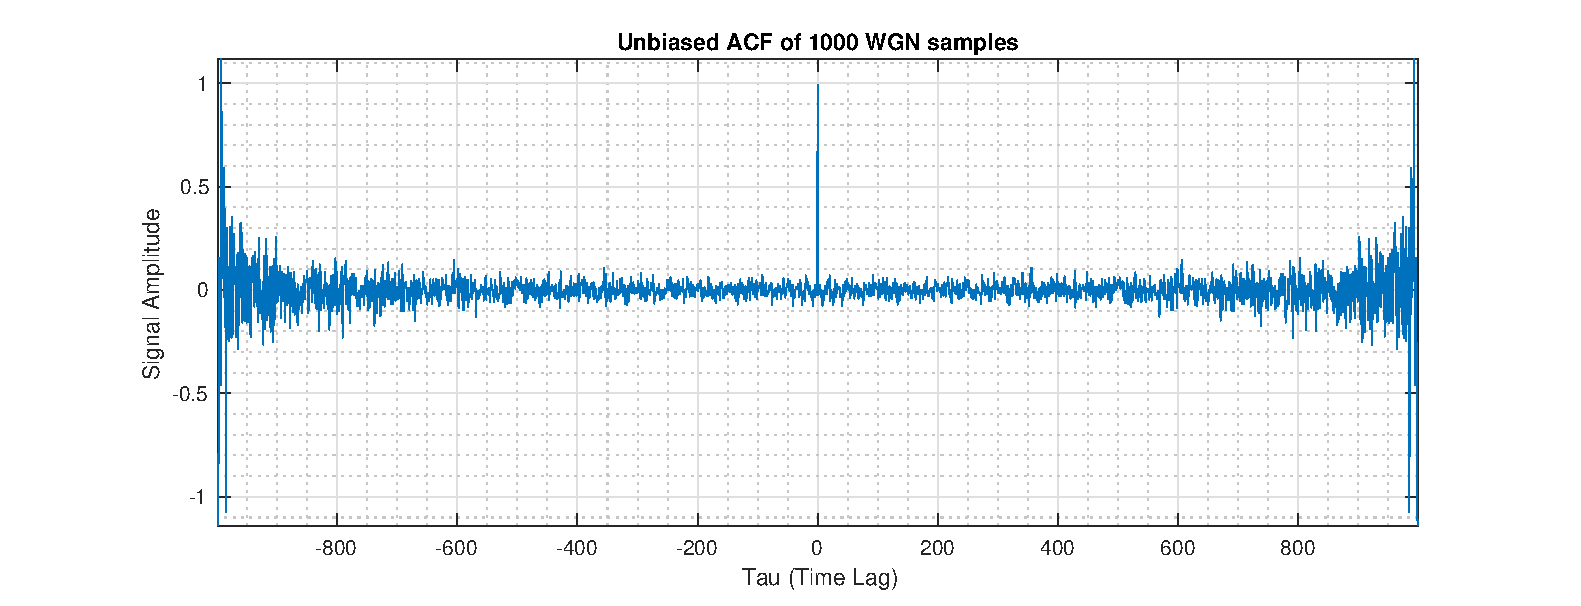
\includegraphics[width=0.6\textwidth]{acf_uncorr}
\caption{\label{fig:acf_uncorr} Unbiased autocorrelation of White Gaussian Noise}
\end{figure}

Figure \ref{fig:acf_uncorr} shows the autocorrelation function of 1000 random White Gaussian Noise (WGN) samples. The function is symmetric about $\tau=0$ since the signal is real. Ideally, the WGN samples would be random and hence completely uncorrelated, so the ACF would have a Dirac delta function at $\tau=0$ and be 0 everywhere else. There is a Dirac delta signal at $\tau=0$ since the signal is perfectly correlated, but the ACF is not zero everywhere else. The cross correlation estimate is close to 0 around $\tau=0$ and increases after $\tau=500$. This is because less than half the signal (of length 1000) is available for comparison and there is a greater error in the estimate. Therefore, the amplitude of the estimate increases as the signal length compared decreases towards $\tau=1000$.

\subsubsection{Zooming in on $\tau=0$}

\begin{figure}[h!]
\centering
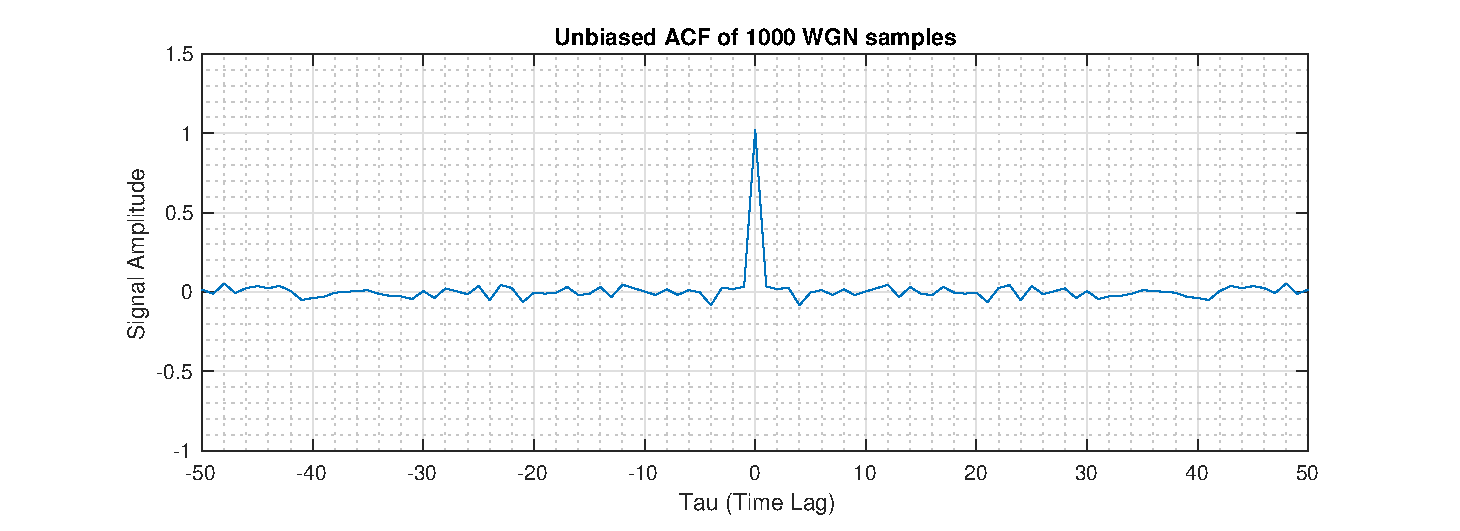
\includegraphics[width=0.6\textwidth]{acf_uncorr_zoom}
\caption{\label{fig:acf_uncorr_zoom} Zooming in to observe the ACF near $\tau=0$}
\end{figure}

Figure \ref{fig:acf_uncorr_zoom} shows the cross correlation estimate is almost identical to the ideal case around $\tau=0$. However, for large $\tau$, the ACF estimate is much larger and becomes higher than the peak of 1 close to $\tau=\pm 999$.

\subsubsection{Effects of large lag $\tau$}

\begin{equation}
\hat{R_{x,unbiased}(\tau)}=\frac{1}{N-|\tau|} \sum_{n=0}^{N-|\tau|-1} x[n]x[n+\tau]
\label{eq:acf}
\end{equation}

We know from Equation \ref{eq:acf} that the autocorrelation estimator's output increases when the number of samples available for comparison decreases. This happens when $\tau$ increases. This makes sense intuitively since the chances for compared samples to be identical increases when the number of samples decreases. We said earlier that the estimator begins diverging roughly after $\tau=\pm500$, so a conservative empirical bound would be half this value, i.e, $\tau=250$. In the general case, the bound would be $\frac{N}{4}$.

\subsubsection{Using a Moving Average Filter}

\begin{figure}[h!]
\centering
\begin{subfigure}{0.32\textwidth}
\centering
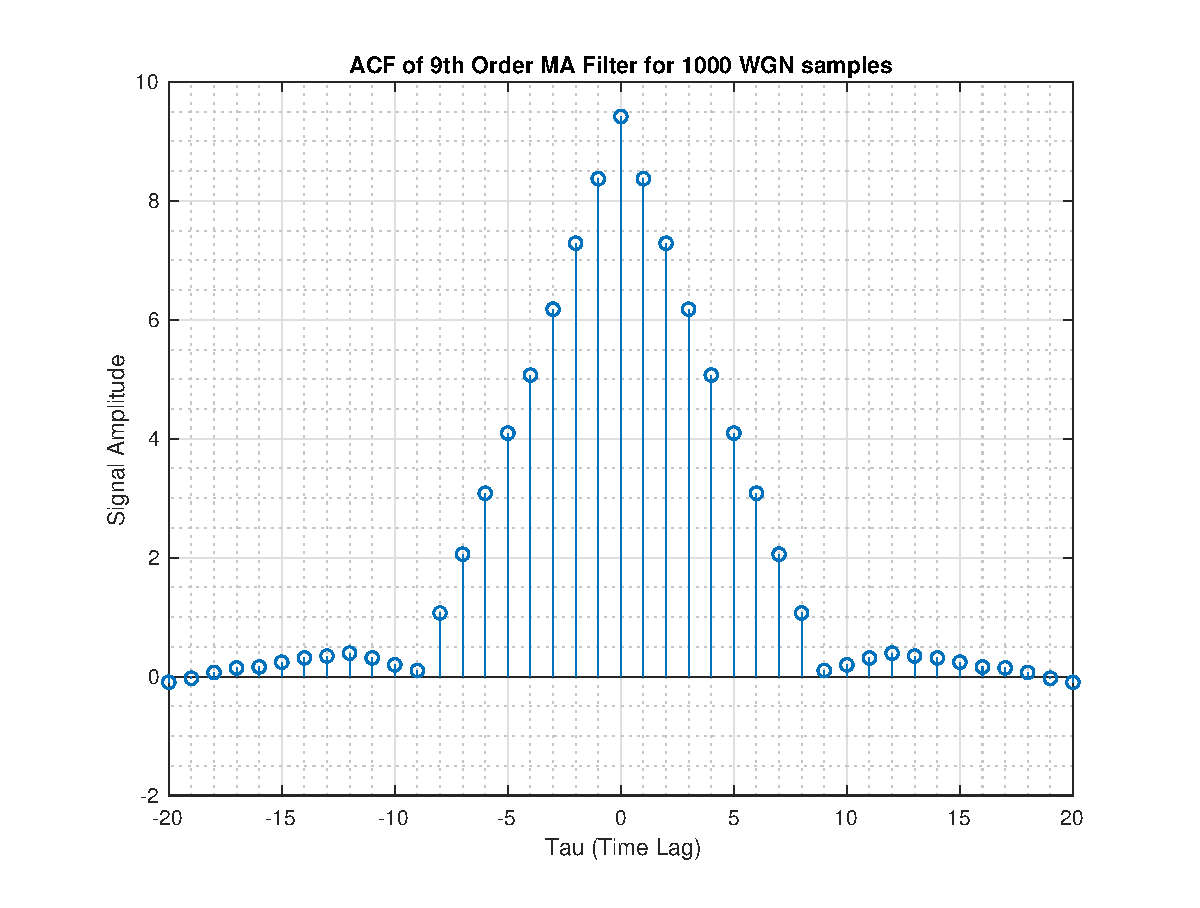
\includegraphics[width = \textwidth]{acf_corr_9}
\caption{9th Order Filter}
\label{fig:acf_corr_9}
\end{subfigure}
\begin{subfigure}{0.32\textwidth}
\centering
\includegraphics[width = \textwidth]{acf_corr_4}
\caption{4th Order Filter}
\label{fig:acf_corr_4}
\end{subfigure}
\caption{Comparing the ACF of Moving Average Filter outputs for different orders}
\label{fig:acf_corr}
\end{figure}

Figure \ref{fig:acf_corr} shows the effects of applying an $N^{th}$ order Moving Average Filter to 1000 WGN samples. The ideal ACF output for an $N^{th}$ order MA filter should be $ACF(\tau) = N \cdot \bigwedge(\frac{\tau}{N})$, where $\bigwedge(t)$ is the triangle function. Figure \ref{fig:acf_corr_9} shows that the ACF of a $9^{th}$ order filter is the triangular function between $-8<\tau<8$. While the ACF should ideally be 0 for $\tau$ outside this range, we see non zero values since we are using an estimate. Decreasing the filter order to 4 decreases the width and height of the triangle, and we can expect a scaling up if the order is increased.\\

An FIR filter can be described by the equation $y[n]=\sum_{i=0}^{N-1}b_ix[n-i]$, where N is the filter order. If all the coefficients are $\frac{1}{N}$, then $y[n]=\frac{1}{N} \sum_{i=0}^{N-1}x[n-i]$. This is equal to the local sample $\hat{m}$. Note that the number of samples must be at least as large as the filter order for a good estimate.

\subsubsection{Correlation of a stochastic process}

\begin{equation}
R_Y(\tau)=R_X{\tau} \ast R_h(\tau)
\end{equation}

where $X_n$ is an uncorrelated process and $Y_n$ is a filtered version of $X_n$. Since $X_n$ is an uncorrelated process, $R_X(\tau)=\alpha \delta(\tau) \Rightarrow R_Y(\tau)=\alpha R_h(\tau)$ since the convolution of any function with the delta function is equal to itself. Thus the ACF of Y is equal to a scaled version of the ACF of the impulse response, which in this case is $N \cdot \bigwedge(\frac{\tau}{N})$.

\vspace{0.5cm}

\subsection{Cross correlation function}

\subsubsection{Cross correlation of X and Y from 2.2}

\begin{figure}[h!]
\centering
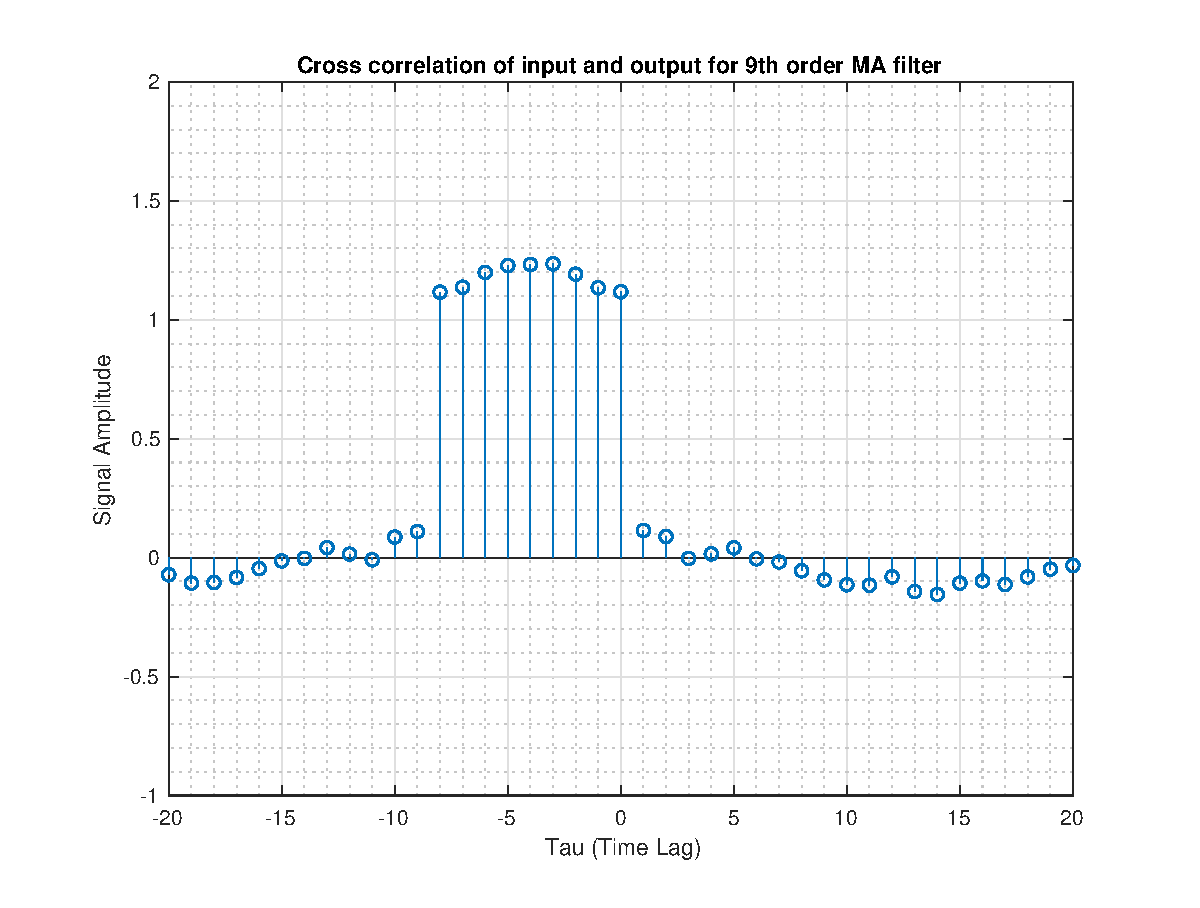
\includegraphics[width=0.33\textwidth]{crosscorr}
\caption{\label{fig:crosscorr} Cross correlation of input and output for 9th order MA filter}
\end{figure}

Figure \ref{fig:crosscorr} shows that X is correlated to the current and last 8 values of Y. This is expected since the filter order is 9. Since $X_n$ is uncorrelated, $R_{XY}(\tau)=h(\tau) \ast R_X(\tau)=h(\tau) \ast \delta (t) = h(\tau)$. In this case, $h(\tau)$ is the pulse train represented by $\sum_{i=0}^N \delta(\tau - i)$.

\subsubsection{Application to System Identification}

If we cross correlate a function with its output through any LTI system, we can obtain the impulse response of the system as long as the original function is uncorrelated. The order of the filter can then be deduced by the number of delta peaks in the impulse response. The coefficients can also be estimated if the system is an FIR. Thus system identification can be conducted by observing any of these characteristic properties.

\pagebreak


\subsection{Autoregressive Modelling}

\subsubsection{Stability of coefficients for AR(2)}

AR(2) is defined as:

\begin{equation}
x[n] = a_1 x[n-1] + a_2 x[n-2] + w[n] \text{,   where } w[n] \sim N(0,1)
\end{equation}
\\
Figure \ref{fig:autoreg} shows the stable and unstable coefficient pairs ($a_1$,$a_2$) in the blue and red regions respectively. The response will be bounded (i.e WSS) within the blue region. The roots will diverge outside the stable region and the mean will vary (i.e not WSS).

\begin{figure}[h!]
\centering
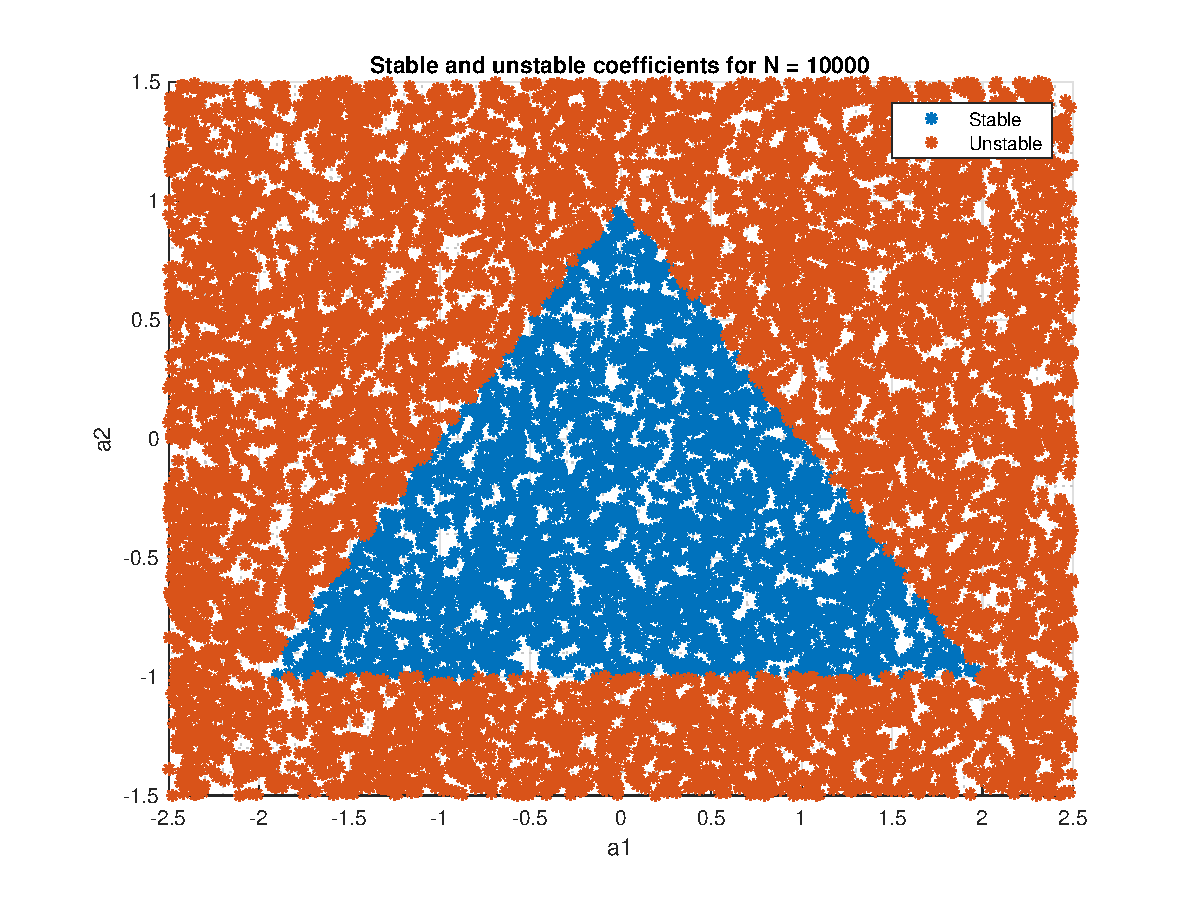
\includegraphics[width=0.5\textwidth]{autoreg}
\caption{\label{fig:autoreg} Stability of coefficients $a_1$ and $a_2$}
\end{figure}

The system's poles must lie within the unit circle for stability. The roots of the characteristic equation $C(z)=z^2 -a_1 z - a_2$ are $z=\frac{a_1 \pm \sqrt[]{a_1^2 + 4a_2}}{2}$. For the positive root, we have:

\begin{align*}
\frac{a_1 \pm \sqrt[]{a_1^2 + 4a_2}}{2} &< 1\\
a_1^2 + 4a_2 &< (2-a_1)^2\\
a_1^2 + 4a_2 &< 4 + a_1^2 - 4a_1\\
a_1 + a_2 &< 1
\end{align*}
Similar calculations for the negative root give $a_2-a_1<1$.\\

The characteristic equation can now be written as:
\begin{align*}
C(z) &= (z-\lambda_1)(z-\lambda_2) = 0\\
&= z^2-(\lambda_1 + \lambda_2)z + \lambda_1\lambda_2=0\\
\therefore a_1 &= (\lambda_1 + \lambda_2)\\
a_2 &= \lambda_1\lambda_2
\end{align*}
Since both roots are less than 1, $|a_2|<1$.\\

Thus the triangular plane of stability is defined by following inequalities:
\begin{align}
\centering
a_1 + a_2 &< 1\\
a_1 - a_2 &< 1\\
|a_2|&<1
\end{align}

\pagebreak

\subsubsection{Sunspot Time Series}

We cannot see any recurrence in the ACF of sunspot data for N=5 (see Figure \ref{fig:sunspot_acf_5}), but can observe the pattern repeating about every 13 years for N=20 (See Figure \ref{fig:sunspot_acf_20}). The ACF with 250 samples has irregularities (see Figure \ref{fig:sunspot_acf_250}) due to the number of samples being greater than the empirical bound of $N/4$ discussed earlier. If we stay within this bound, we see the perfect sinusoid pattern shown in Figure \ref{fig:sunspot_acf_250_zoom}.\\

The zero mean version provides equal representation for positive and negative elements and prevents a build up of the product of shifted elements. This reveals a clearer picture of the underlying trends in the sunspot data. For example, the ACF of sunspot data for N=20 would suggest that the signal is more similar to itself when it is shifted, which is obviously incorrect. Standardizing the data removes this problem. It also makes the periodicity of data for N=5 and N=250 more clear.


\begin{figure}[h!]
\centering
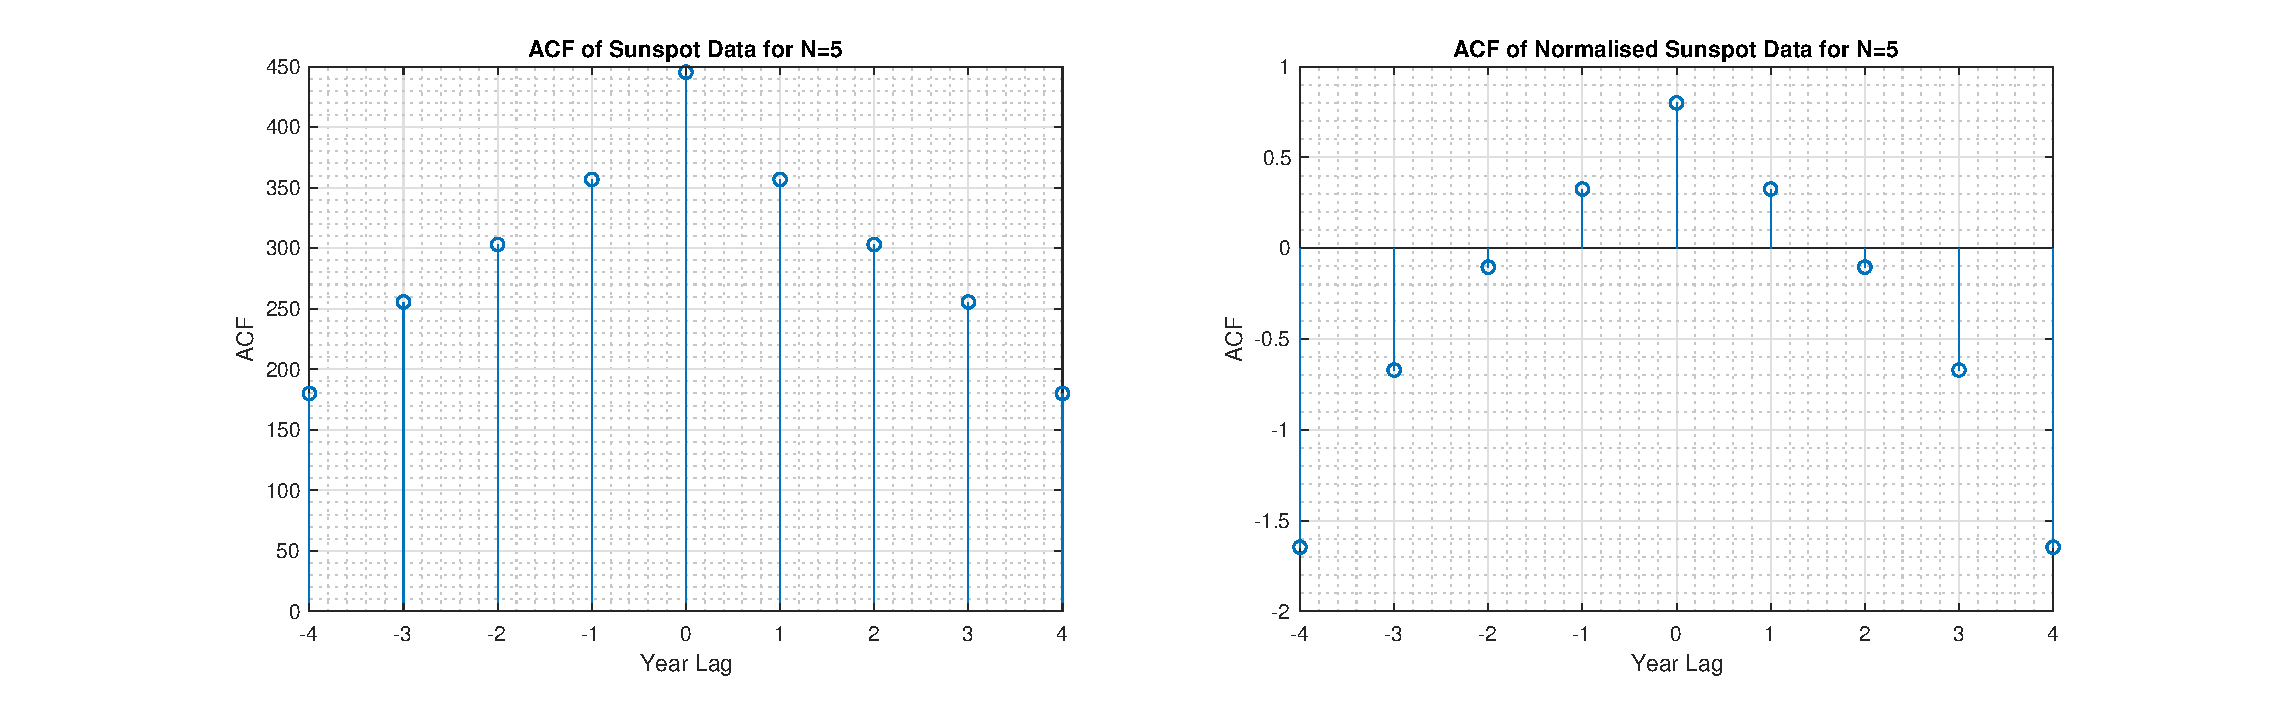
\includegraphics[width = 0.66\textwidth]{sunspot_acf_5}
\caption{ACF of sunspot data with data length N=5}
\label{fig:sunspot_acf_5}
\end{figure}

\begin{figure}[h!]
\centering
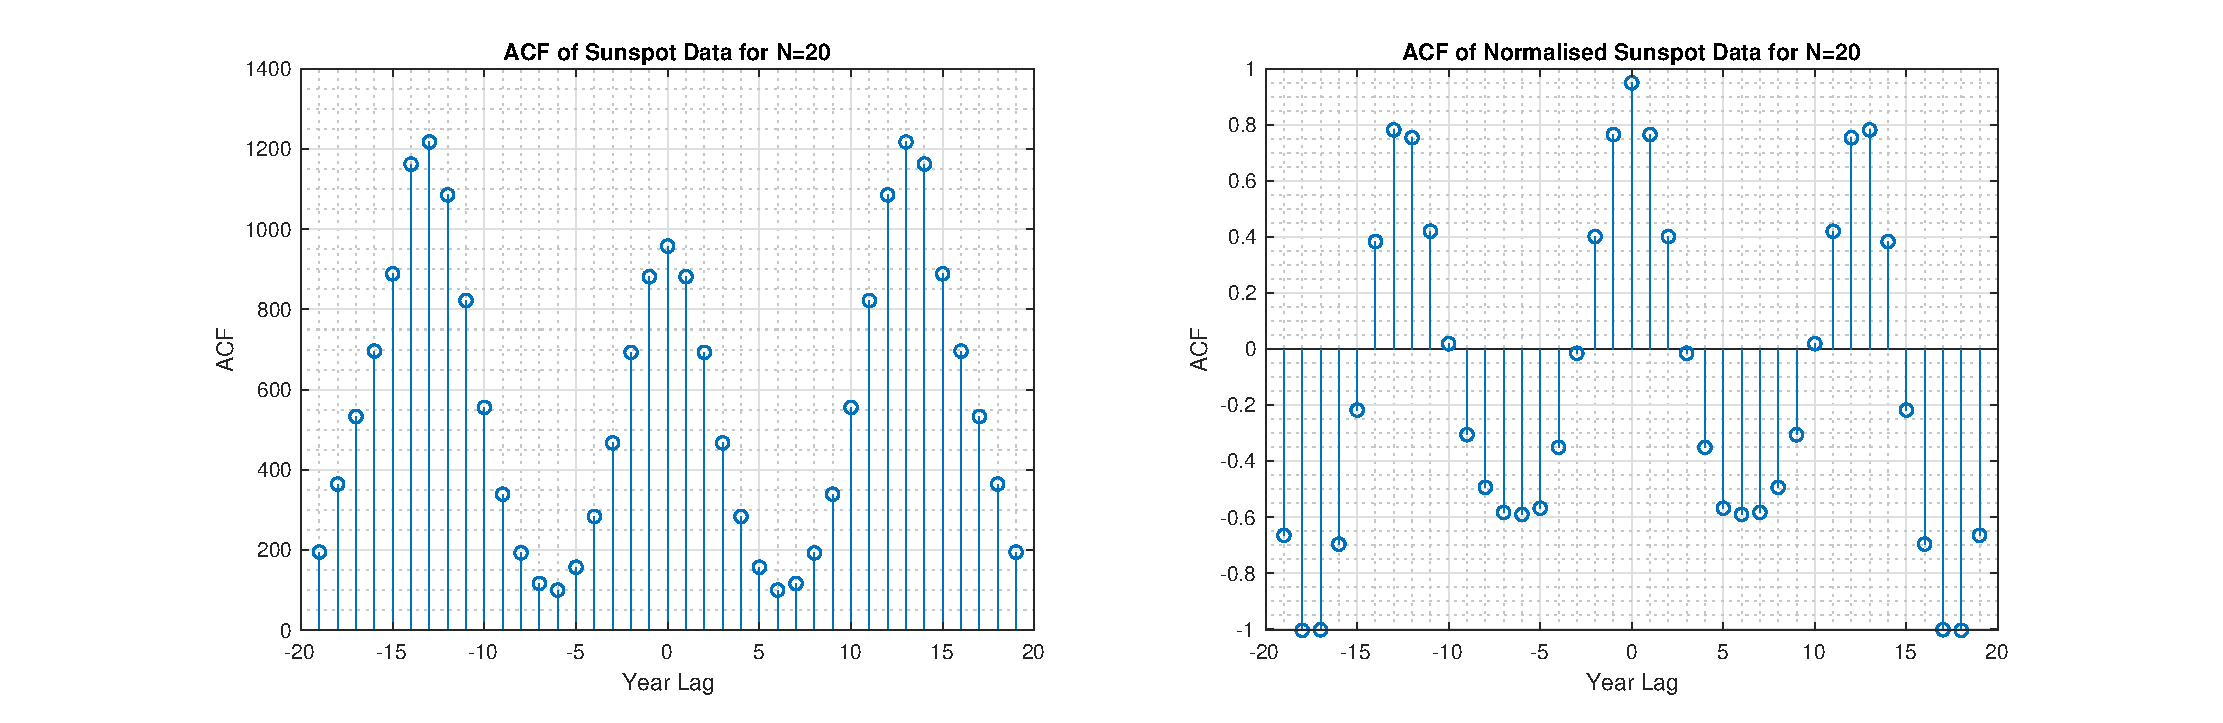
\includegraphics[width = 0.66\textwidth]{sunspot_acf_20}
\caption{ACF of sunspot data with data length N=20}
\label{fig:sunspot_acf_20}
\end{figure}

\begin{figure}[h!]
\centering
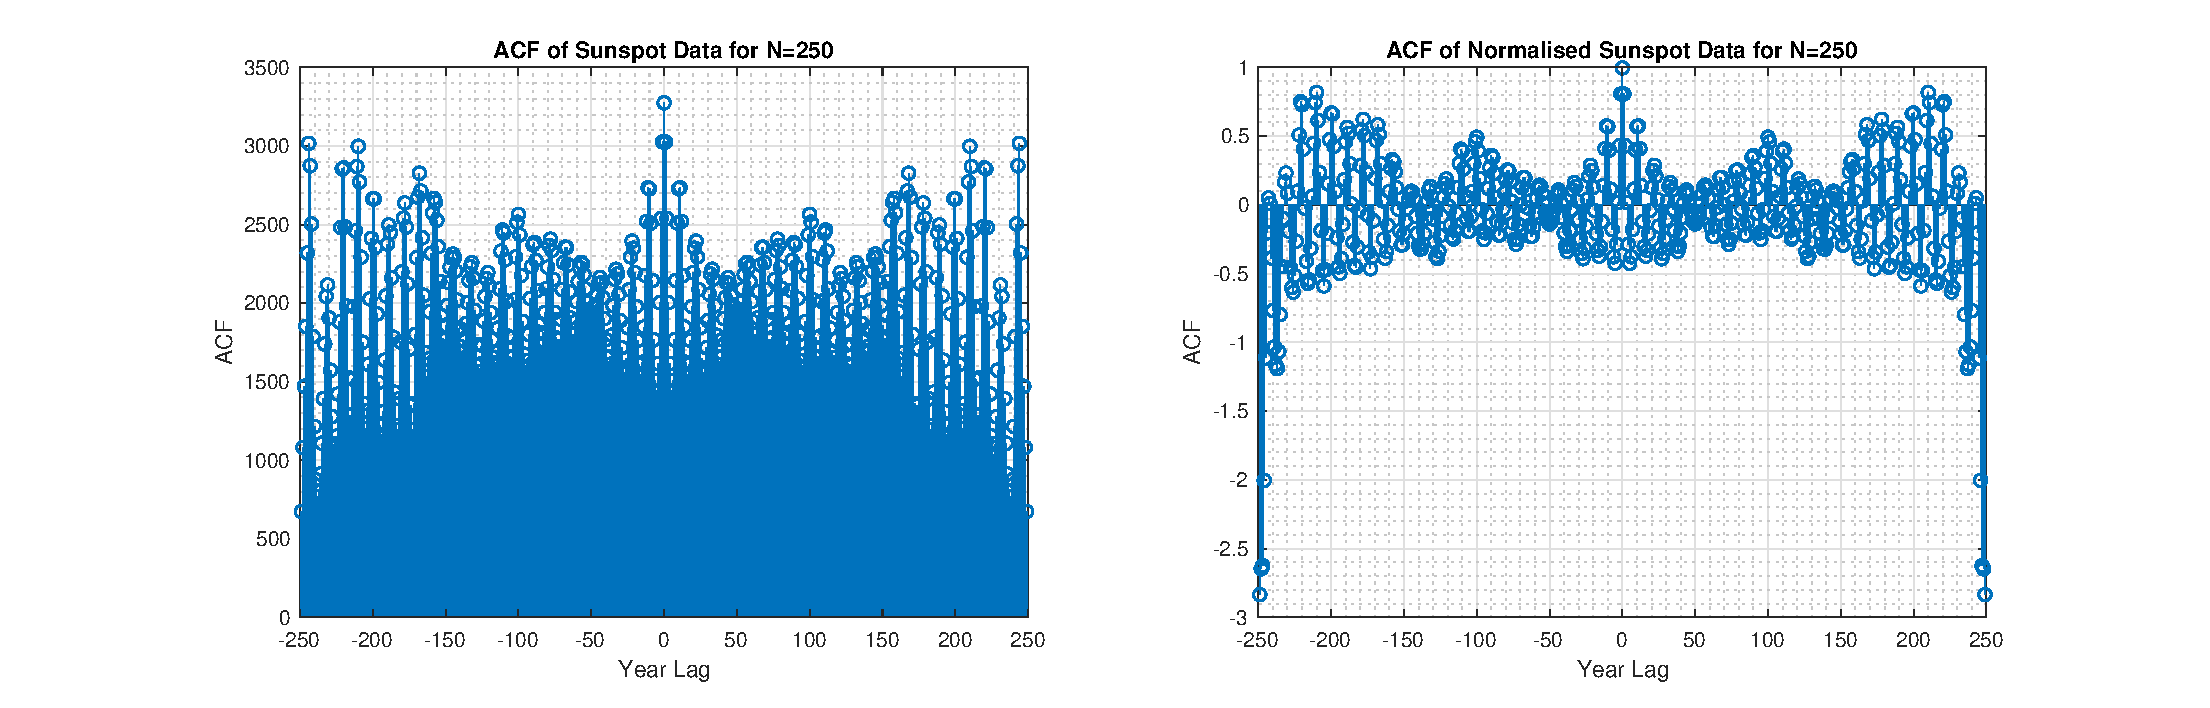
\includegraphics[width = 0.66\textwidth]{sunspot_acf_250}
\caption{ACF of sunspot data with data length N=250}
\label{fig:sunspot_acf_250}
\end{figure}

\begin{figure}[h!]
\centering
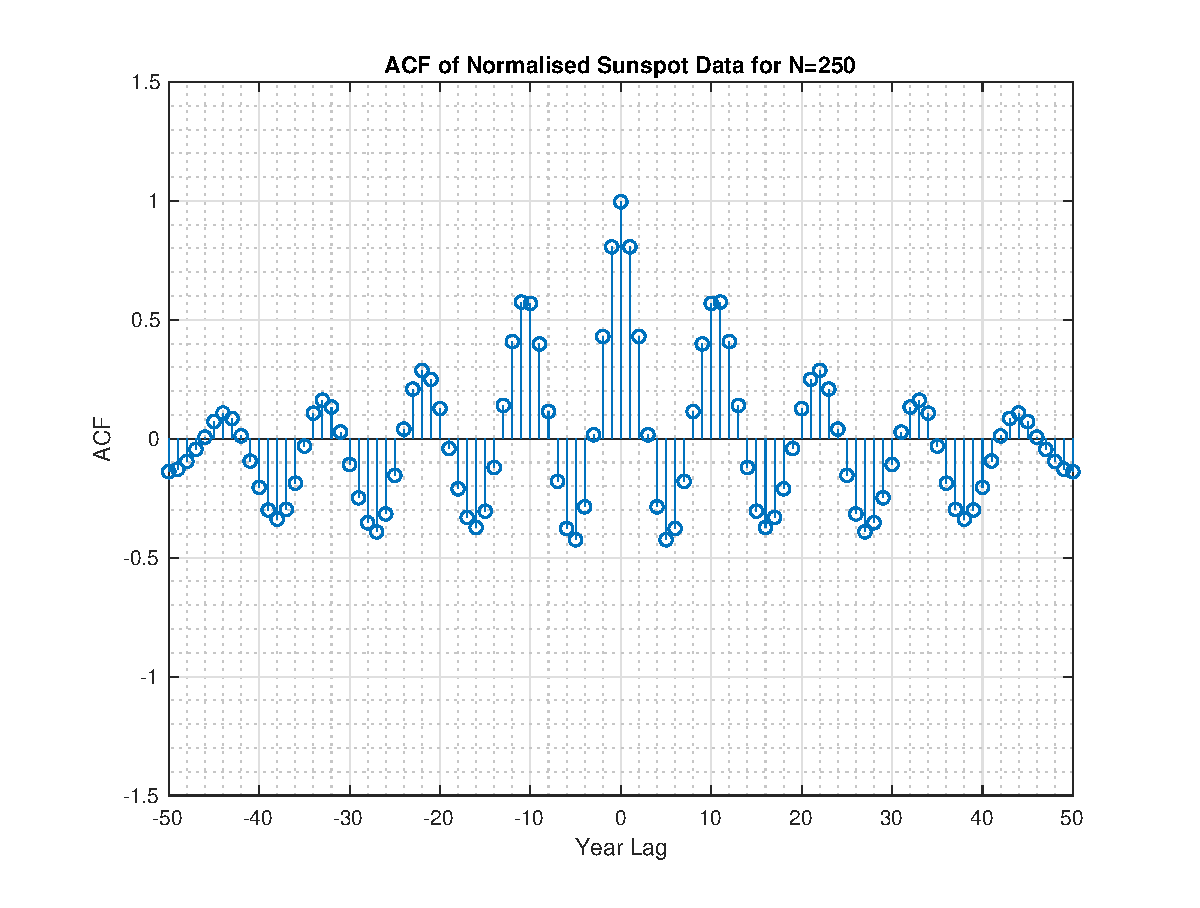
\includegraphics[width = 0.33\textwidth]{sunspot_acf_250_zoom}
\caption{Zooming into the normalized ACF with N=250 shows a sinusoidal pattern}
\label{fig:sunspot_acf_250_zoom}
\end{figure}

\pagebreak

\subsubsection{The Yule Walker Equations and Partial Correlation}

Figure \ref{fig:yulewalker} clearly shows that the best model order is 2 since the coefficients for all others converge to 0. Figure \ref{fig:pcf} illustrates the difference between the regular and standardized partial correlation function (PCF). The standardized version is more accurate since it removes any offsets that obscure underlying trends. The significant decrease in the PCF after order 2 indicates that the current sunspot sample has weak correlation with the sample 3 time units ago. This property defines the AR(2) process.

\begin{figure}[h!]
\centering
\begin{subfigure}{0.32\textwidth}
\centering
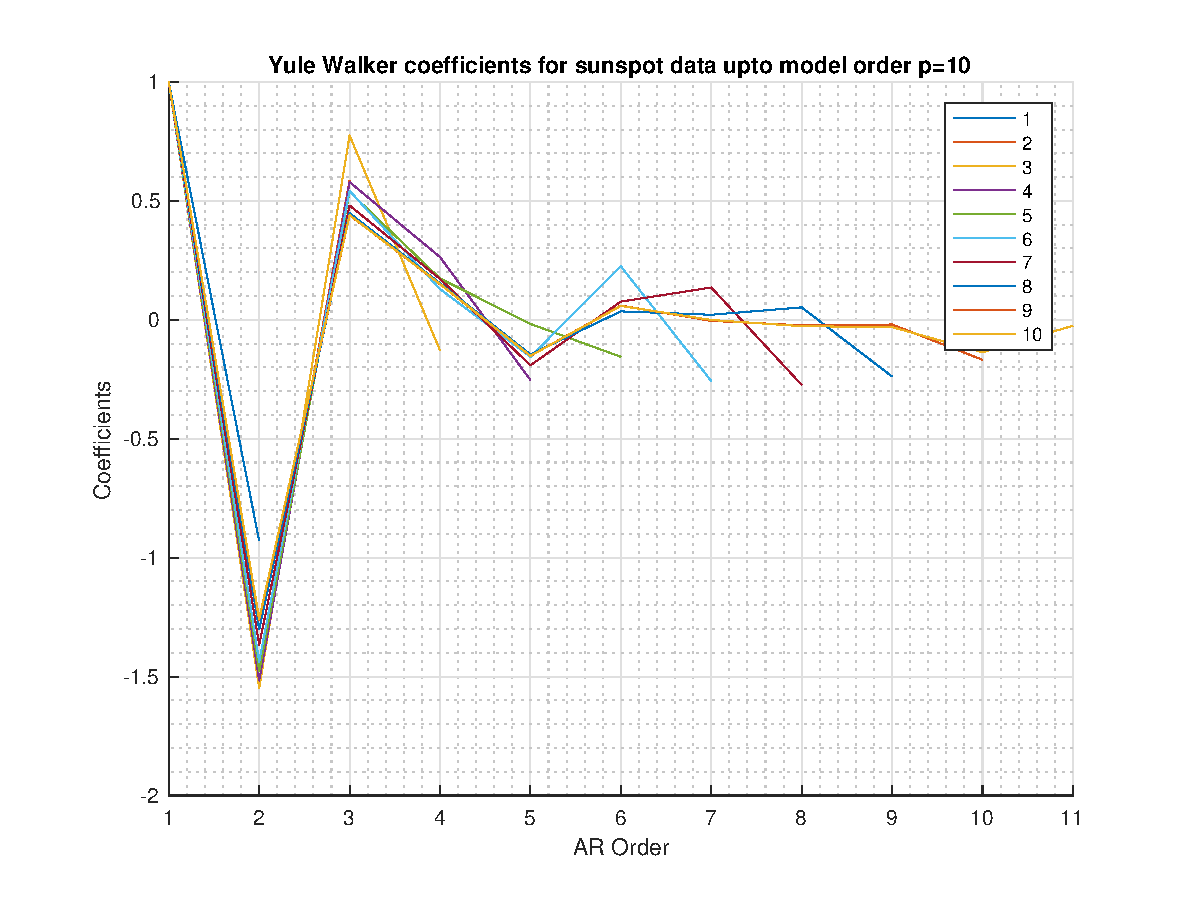
\includegraphics[width = \textwidth]{yulewalker}
\caption{Yule Walker coefficients}
\label{fig:yulewalker}
\end{subfigure}
\begin{subfigure}{0.32\textwidth}
\centering
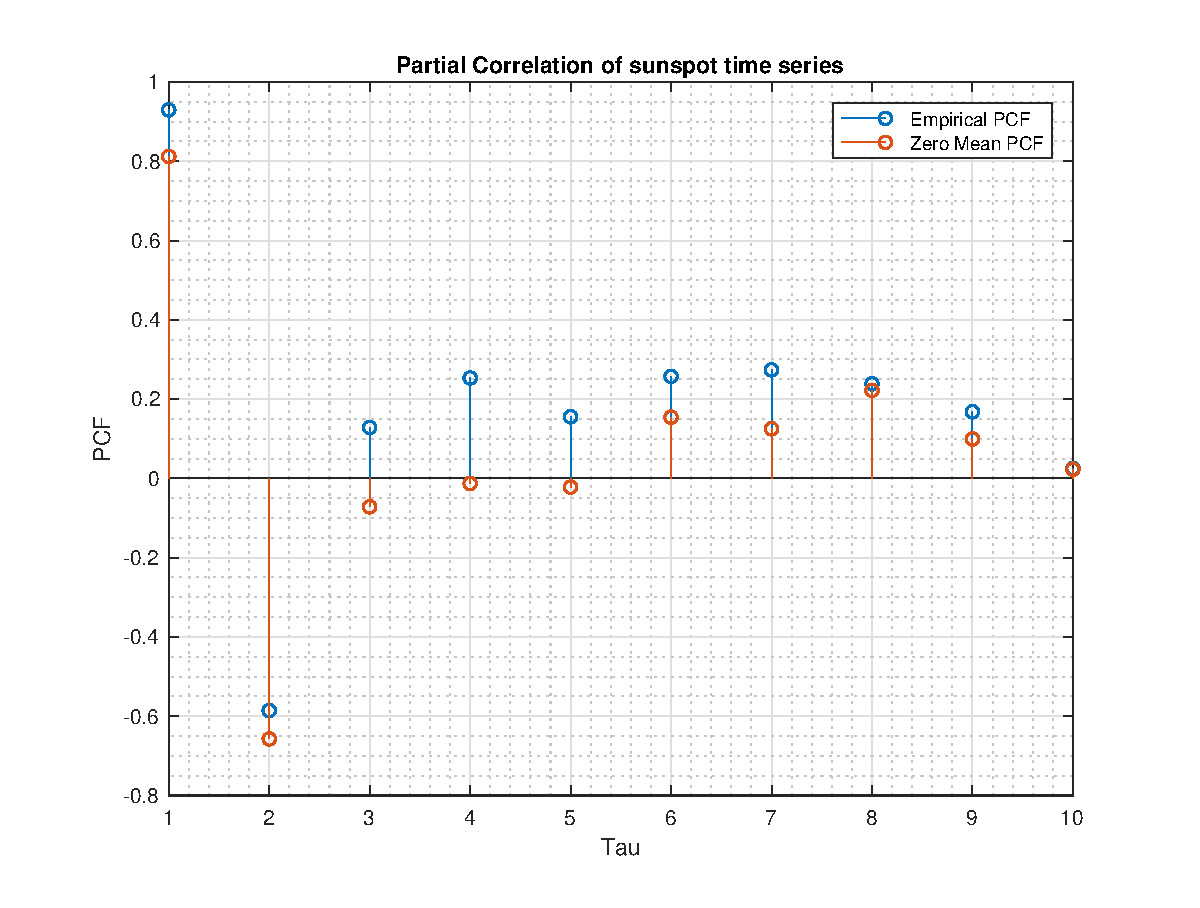
\includegraphics[width = \textwidth]{pcf}
\caption{Partial correlation function}
\label{fig:pcf}
\end{subfigure}
\label{yule_pcf}
\caption{}
\end{figure}


\subsubsection{Determining the correct model order}

\begin{figure}[h!]
\centering
\begin{subfigure}{0.32\textwidth}
\centering
\includegraphics[width = \textwidth]{mdl_aic_zoom}
\caption{MDL, AIC, Loss function}
\label{fig:mdl_aic_zoom}
\end{subfigure}
\begin{subfigure}{0.32\textwidth}
\centering
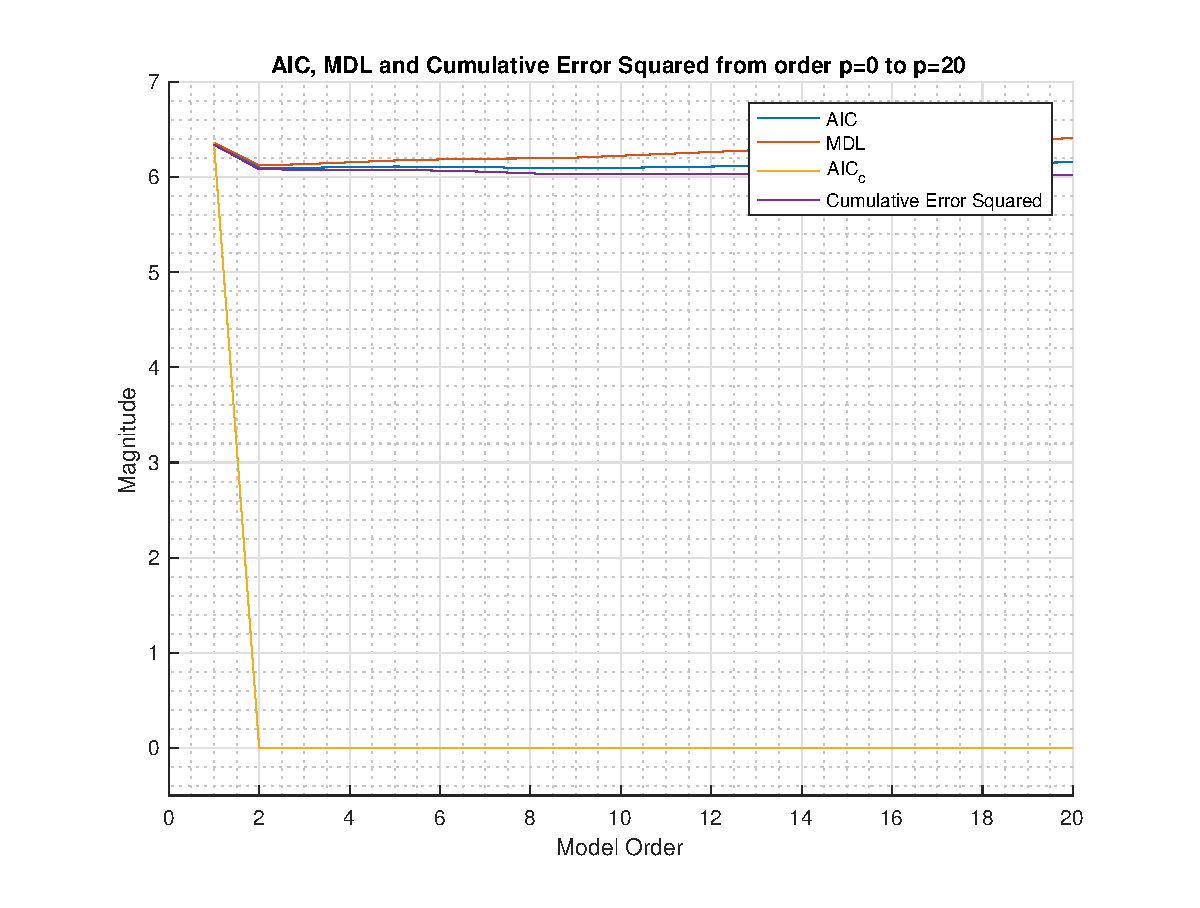
\includegraphics[width = \textwidth]{mdl_aic}
\caption{Zooming out for $AIC_c$}
\label{fig:mdl_aic}
\end{subfigure}
\caption{Selection criteria for model order}
\label{yule_pcf}
\end{figure}

The purpose of using the Minimum Description Length (MDL), Akaike Information Criterion (AIC) and cumulative error squared is to balance the reduction in error with the increase in complexity. Since the loss function will always decrease when the order is increased, the MDL and AIC increase their respective magnitudes for higher orders, thus providing a guide to prevent unnecessary increases in the applied model order.\\

While the global minimum in Figure \ref{fig:mdl_aic} occurs at p=9, the first minimum occurs at p=2. Since the drop in error between the two orders is only about 0.055, the sunspot time series should be modeled as a second order autoregressive process. AR(1) clearly follows the real sunspot data for one horizon (i.e m=1) but deviates for m=2, m=5 and m=10.

\pagebreak

\subsubsection{AR Modeling to predict the sunspot time series}

We now compare the the AR(1),AR(2) and AR(10) models to see which one can predict the sunspot time series best. Figure \ref{fig:ar_mod_hor} clearly shows that increasing the model order allows for a more accurate prediction. All 3 orders display a fall in amplitude with increase in horizon, which means AR(1) and AR(2) are unsuitable for estimating the sunspot data over a long horizon. Increasing the order from AR(1) to AR(2) decreases the lag between the estimate and the real data. However, as discussed earlier, this increases the number of variables required for computation and hence raises the complexity of calculations involved.


\begin{figure}[h!]
\centering
\begin{subfigure}{0.24\textwidth}
\centering
\includegraphics[width = \textwidth]{ar_mod1_hor1}
\caption{P=1, M=1}
\label{fig:ar_mod1_hor1}
\end{subfigure}
\begin{subfigure}{0.24\textwidth}
\centering
\includegraphics[width = \textwidth]{ar_mod1_hor2}
\caption{P=1, M=2}
\label{fig:ar_mod1_hor2}
\end{subfigure}
\begin{subfigure}{0.24\textwidth}
\centering
\includegraphics[width = \textwidth]{ar_mod1_hor5}
\caption{P=1, M=5}
\label{fig:ar_mod1_hor5}
\end{subfigure}
\begin{subfigure}{0.24\textwidth}
\centering
\includegraphics[width = \textwidth]{ar_mod1_hor10}
\caption{P=1, M=10}
\label{fig:ar_mod1_hor10}
\end{subfigure}
\begin{subfigure}{0.24\textwidth}
\centering
\includegraphics[width = \textwidth]{ar_mod2_hor1}
\caption{P=2, M=1}
\label{fig:ar_mod2_hor1}
\end{subfigure}
\begin{subfigure}{0.24\textwidth}
\centering
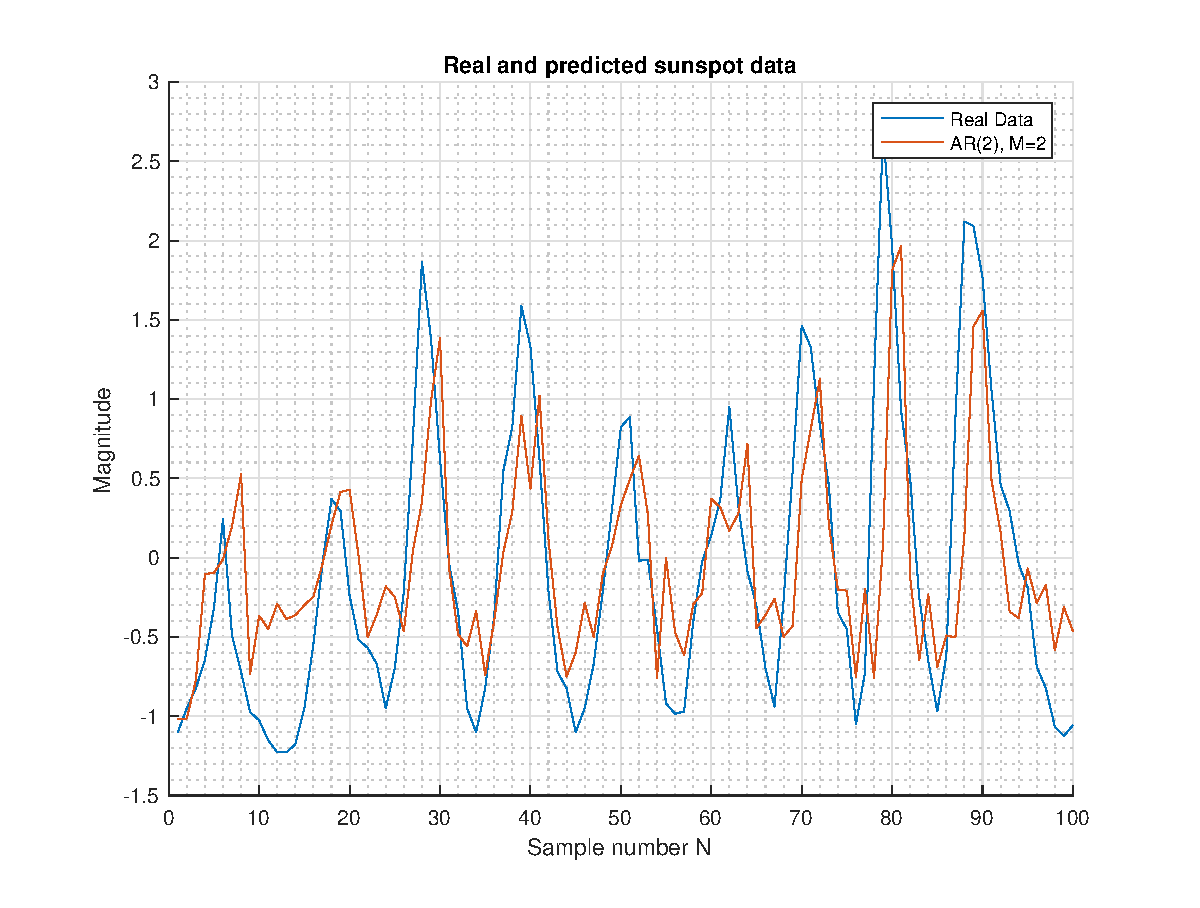
\includegraphics[width = \textwidth]{ar_mod2_hor2}
\caption{P=2, M=2}
\label{fig:ar_mod2_hor2}
\end{subfigure}
\begin{subfigure}{0.24\textwidth}
\centering
\includegraphics[width = \textwidth]{ar_mod2_hor5}
\caption{P=2, M=5}
\label{fig:ar_mod2_hor5}
\end{subfigure}
\begin{subfigure}{0.24\textwidth}
\centering
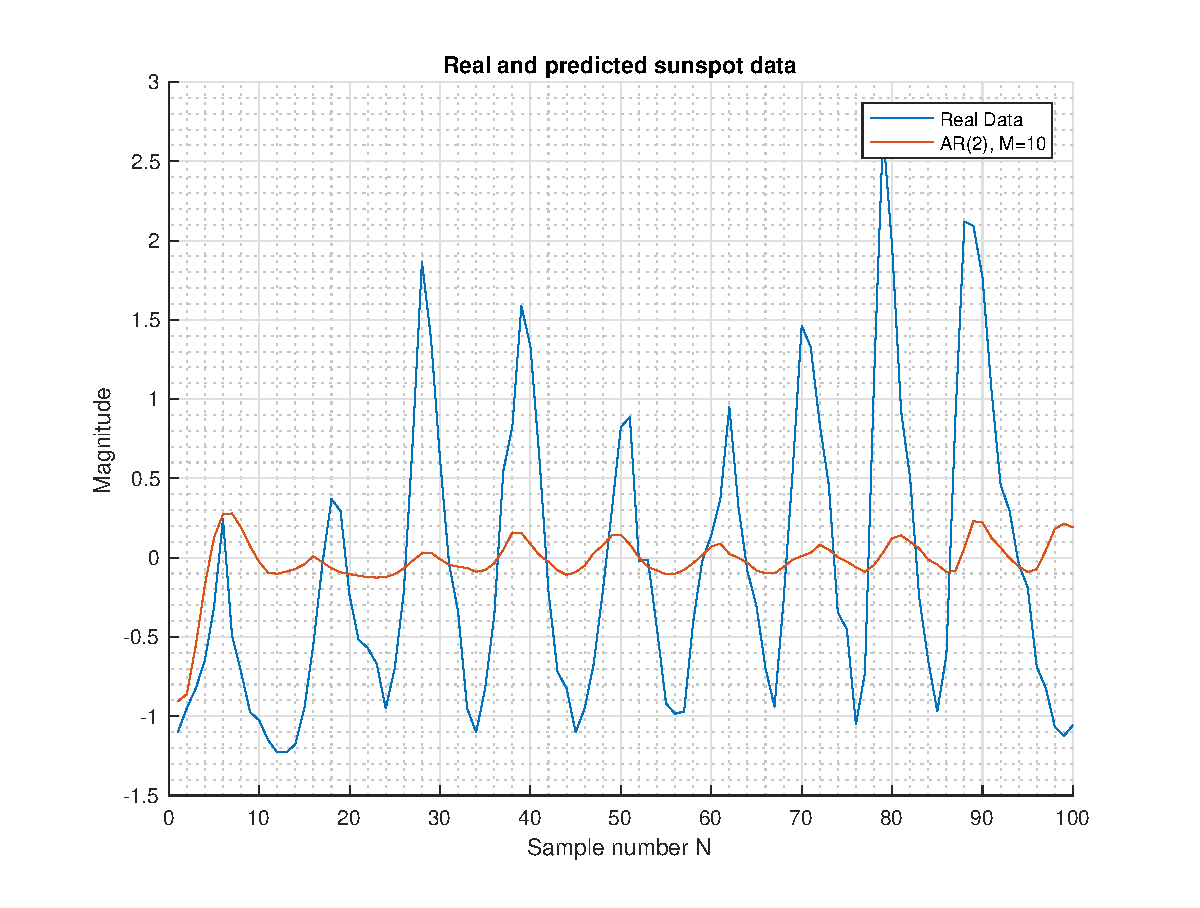
\includegraphics[width = \textwidth]{ar_mod2_hor10}
\caption{P=2, M=10}
\label{fig:ar_mod2_hor10}
\end{subfigure}
\begin{subfigure}{0.24\textwidth}
\centering
\includegraphics[width = \textwidth]{ar_mod10_hor1}
\caption{P=10, M=1}
\label{fig:ar_mod10_hor1}
\end{subfigure}
\begin{subfigure}{0.24\textwidth}
\centering
\includegraphics[width = \textwidth]{ar_mod10_hor2}
\caption{P=10, M=2}
\label{fig:ar_mod10_hor2}
\end{subfigure}
\begin{subfigure}{0.24\textwidth}
\centering
\includegraphics[width = \textwidth]{ar_mod10_hor5}
\caption{P=10, M=5}
\label{fig:ar_mod10_hor5}
\end{subfigure}
\begin{subfigure}{0.24\textwidth}
\centering
\includegraphics[width = \textwidth]{ar_mod10_hor10}
\caption{P=10, M=10}
\label{fig:ar_mod10_hor10}
\end{subfigure}
\caption{Comparing trends across model order and prediction horizon for N=100 samples}
\label{fig:ar_mod_hor}
\end{figure}



\subsection{Cramer-Rao Lower Bound} % NEED TO FINISH!!

\subsubsection{Sufficiency of an AR(1) model}

Figure \ref{fig:cramer_ar1} shows that the error is minimum for MDL, AIC and the loss function at p=1. Since the NASDAQ data's sample size is no longer small (it is almost 3 times the size of the sunspot data), we can ignore $AIC_c$. The drastic decrease in PCF after order 1 indicates that the NASDAQ data has almost no correlation with the sample more than 1 time unit ago. Thus an AR(1) process is sufficient to model the NASDAQ data.

\begin{figure}[h!]
\centering
\begin{subfigure}{0.32\textwidth}
\centering
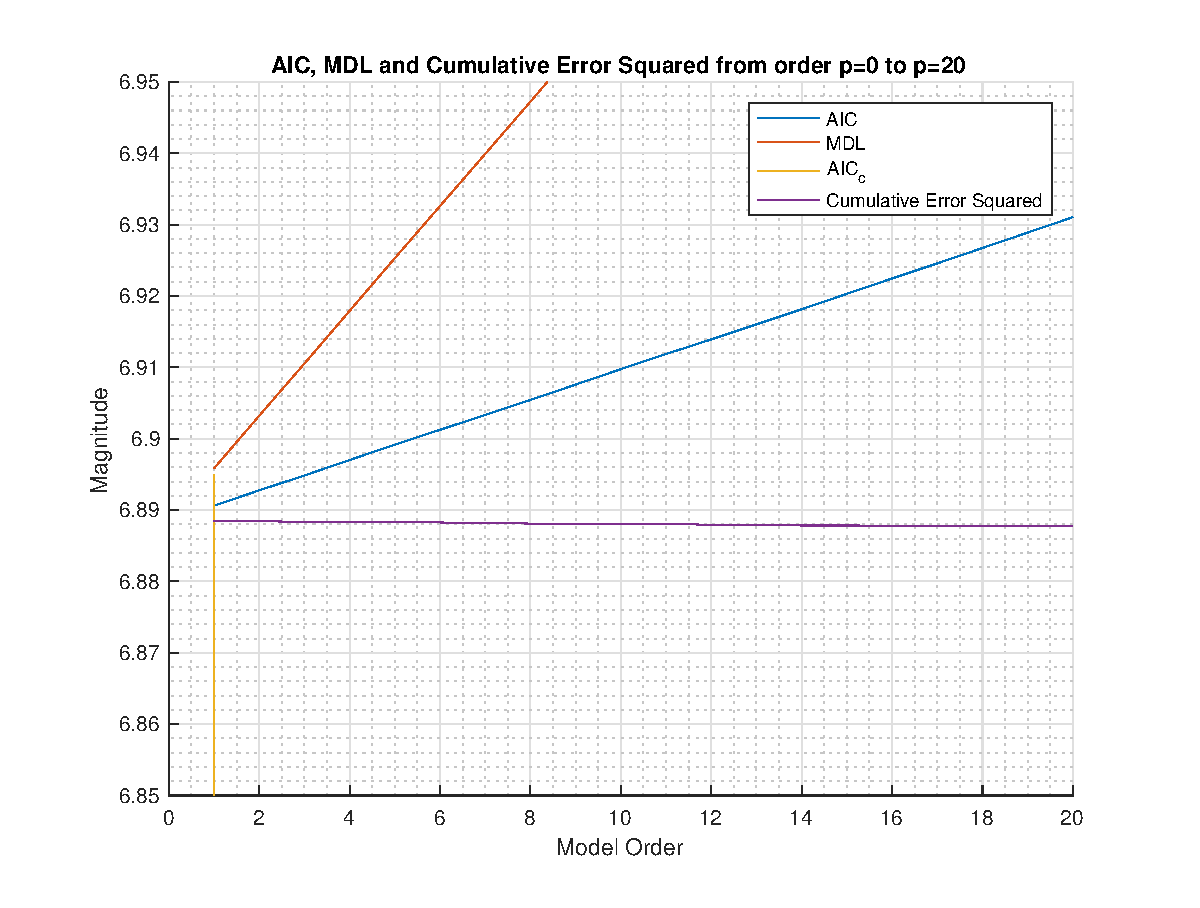
\includegraphics[width = \textwidth]{nasdaq_mdl}
\caption{MDL, AIC, Loss function}
\label{fig:nasdaq_mdl}
\end{subfigure}
\begin{subfigure}{0.32\textwidth}
\centering
\includegraphics[width = \textwidth]{nasdaq_pcf}
\caption{Partial correlation function}
\label{fig:nasdaq_pcf}
\end{subfigure}
\caption{Selection criteria for model order of NASDAQ data}
\label{fig:cramer_ar1}
\end{figure}


\subsubsection{Computing the Fisher Information Matrix}

The following derivations have been sourced from Stephen Kay's 'Fundamentals of Signal Processing: Estimation Theory'. The PSD implied by the AR model is:

\begin{equation}
P_{xx} (f;\theta) = \frac{\sigma_u^2}{|A(f)|^2}
\end{equation}
\\
where $\theta=[a[1] a[a]] \cdots a[p] \sigma_u^2]^T$ and $A(f)=\sum_{m=1}^p a[m] exp(-j2\pi fm)$. The partial derivatives are:

\begin{align}
\frac{\partial ln P_{xx} (f;\theta)}{\partial a[k]} &= -\frac{\partial ln |A(f)|^2}{\partial a[k]}\\
&= -\frac{1}{|A(f)|^2} [A(f)exp(j2\pi fk)+A^*(f)exp(-j2\pi fk)]\\
\frac{\partial ln P_{xx} (f;\theta)}{\partial \sigma_u^2} &= \frac{1}{\sigma_u^2}
\end{align}
\\
For $k = 1,2,...p$ and $l=1,2,...p$, we have:

\begin{equation*}
I[\theta]_{kl} = \frac{N}{2}\int_{-0.5}^{0.5}\frac{1}{|A(f)|^4} [A(f)exp(j2\pi fk)+A^*(f)exp(-j2\pi fk)] \times [A(f)exp(j2\pi fl)+A^*(f)exp(-j2\pi fl)] df
\end{equation*}

\begin{equation}
= \frac{N}{2}\int_{-0.5}^{0.5} \frac{1}{A^*(f)^2} exp(j2\pi f(k+l)) + \frac{1}{|A(f)|^2} exp(j2\pi f(k-l) + \frac{1}{|A(f)|^2} exp(j2\pi f(l-k)) + \frac{1}{A^2(f)} exp(-j2\pi f(l+k)) df
\end{equation}
\\
Using the Hermitian property of the integrand ($A(-f)=A^*(f)$), we have 

\begin{align}
\int_{-0.5}^{0.5} \frac{1}{A^*(f)^2} exp(j2\pi f(k+l)) df &= \int_{-0.5}^{0.5} \frac{1}{A^2(f)} exp(-j2\pi f(l+k)) df \\
\int_{-0.5}^{0.5} \frac{1}{|A(f)|^2} exp(j2\pi f(k-l) df &= \int_{-0.5}^{0.5} \frac{1}{|A(f)|^2} exp(j2\pi f(l-k)) df
\end{align}

\begin{equation}
\therefore [I(\theta)]_{kl} = N \int_{-0.5}^{0.5} \frac{1}{A^*(f)^2} exp(j2\pi f(k+l)) + N \int_{-0.5}^{0.5} \frac{1}{|A(f)|^2} exp(j2\pi f(k-l) df
\end{equation}
\\
The second integral is the inverse Fourier transform of $\frac{1}{A^*(f)^2}$ evaluated at $n=k+l>0$. This term is 0 since the sequence is the convolution of 2 anti-causal sequences, i.e,

\begin{equation}
    F^{-1}[\frac{1}{A(f)}]=
    \begin{cases}
      h[n], & n>=0 \\
      0, & n<0
    \end{cases}
  \end{equation}
  
  \begin{equation}
    F^{-1}[\frac{1}{A^*(f)^2}]=
    \begin{cases}
      h[-n] \star h[-n] \\
      0, & n>0
    \end{cases}
  \end{equation}
  
\begin{equation}
therefore [I(\theta)]_{kl} = \frac{N}{\sigma_u^2}r_{xx}(k-l)
\end{equation}

We are given $I_{11}$, $I_{12}$ and $I_{21}$. For $k=p+1$ and $l=p+1$:

\begin{equation}
[I(\theta)]_{kl} = \frac{N}{2} \int_{-0.5}^{0.5} \frac{1}{\sigma_u^4} df = \frac{N}{2\sigma_u^4}
\end{equation}

\begin{equation}
\therefore I(\theta) = 
\begin{bmatrix}
\frac{N}{\sigma_u^2}R_{xx} & 0 \\
0^T & \frac{N}{2\sigma_u^4}
\end{bmatrix}
\end{equation}

where $[R_{xx}]_{ij} = r_{xx}(i-j)$ is a $p \times p$ Toeplitz autocorrelation matrix and 0 is a $p \times 1$ vector of zeros.

\subsubsection{Computing the lower bound of the variance}

Upon inverting the Fisher Information matrix, we get:

\begin{equation}
var(\hat{a[k]}) >= \frac{\sigma_u^2}{N} [R_{xx}^{-1}]_{kk} \text{  for k = 1,2,...p}
\end{equation}

\begin{equation}
var(\hat{\sigma_u^2}) >= \frac{2\sigma_u^4}{N}
\end{equation}

\begin{equation}
\text{Using p = 1,  } (\hat{a[1]}) >= \frac{\sigma_u^2}{Nr_{xx}[0]}
\end{equation}

\begin{equation}
\text{But  } r_{xx}[0] = \frac{\sigma_u^2}{1-a^2[1]}
\end{equation}

\begin{equation}
\text{So that  } var(\hat{a[1]}) >= \frac{1}{N} (1-a^2[1])
\end{equation}

This shows that it is easier to estimate the filter parameter when a[1] is closer to 1 than to 0. Since the pole of the filter is at -a[1], the filter parameters of processes with PSDs having sharp peaks are more easily estimated.

\begin{figure}[h!]
\centering
\begin{subfigure}{0.33\textwidth}
\centering
\includegraphics[width = \textwidth]{heatmap_a1}
\caption{$\hat{a_1}$}
\label{fig:heatmap_a1}
\end{subfigure}
\begin{subfigure}{0.33\textwidth}
\centering
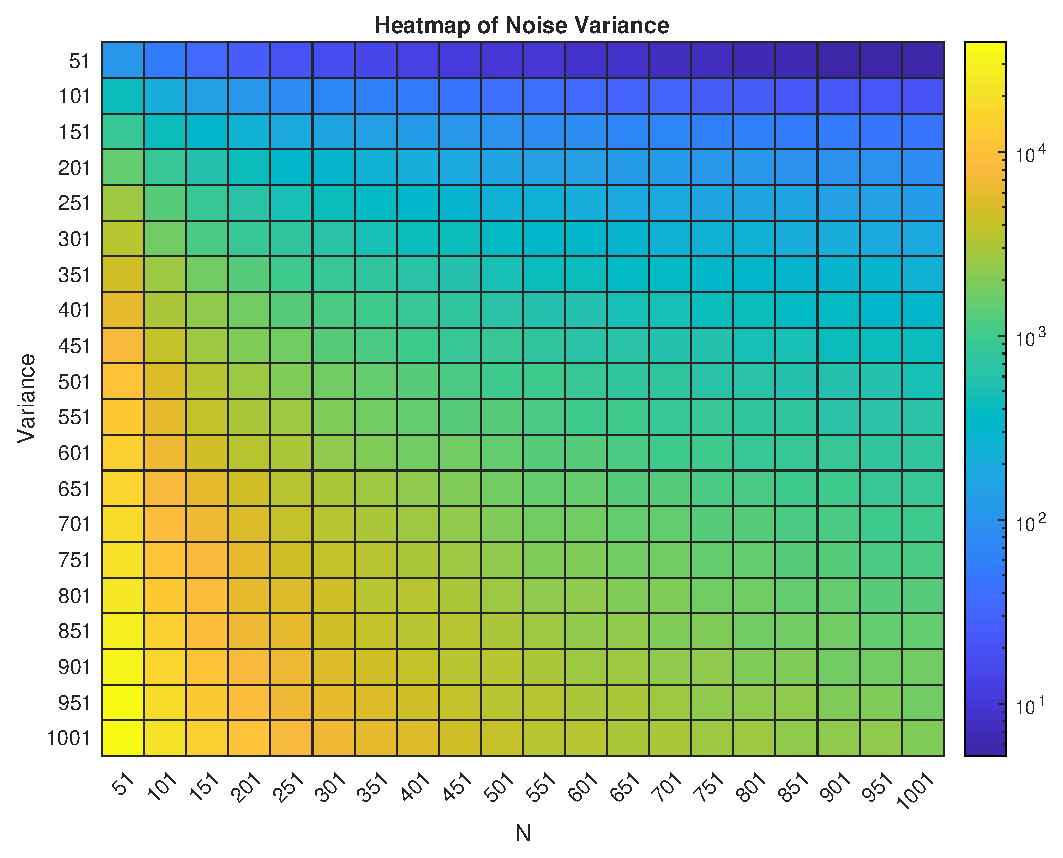
\includegraphics[width = \textwidth]{heatmap_noise}
\caption{Noise variance}
\label{fig:heatmap_noise}
\end{subfigure}
\caption{Cramer Rao lower bound heatmaps for $\hat{\sigma^2}$ and $\hat{a_1}$}
\label{fig:heatmap}
\end{figure}

\subsubsection{Computing the bound in terms of A(f)}

For $p=1$,

\begin{align}
\frac{\hat{P_x(f;\theta)}}{\partial a_1} &= \frac{\sigma^2 [exp(j2\pi f)A(f) + exp(-j2\pi f)A(-f)}{[A(f)A(-f)]^2} \\
&= \frac{\sigma^2 [exp(-j2\pi f) - a_1 + exp(j2\pi f) - a_1]}{|A(f)|^4} \\
&= \frac{2\sigma^2[cos(2\pi f) - a_1]}{|A(f)|^4}
\end{align}

\begin{equation}
\text{and } \frac{\hat{P_x(f;\theta)}}{\partial \sigma^2} = \frac{1}{|A(f)|^2}
\end{equation}

\begin{align}
\therefore var(\hat{P_x(f;\theta)}) &<=
\begin{bmatrix}
\frac{2\sigma^2[cos(2\pi f) - a_1]}{|A(f)|^4} & \frac{1}{|A(f)|^2}
\end{bmatrix}
\begin{bmatrix}
\frac{1-a_1^2}{N} & 0 \\
0 & \frac{2\sigma^4}{N}
\end{bmatrix}
\begin{bmatrix}
\frac{2\sigma^2[cos(2\pi f) - a_1]}{|A(f)|^4} \\
\frac{1}{|A(f)|^2}
\end{bmatrix}
\\
&=
\begin{bmatrix}
\frac{1-a_1^2}{N} \frac{2\sigma^2[cos(2\pi f) - a_1]}{|A(f)|^4} & \frac{2\sigma^4}{N |A(f)|^2}
\end{bmatrix}
\begin{bmatrix}
\frac{2\sigma^2[cos(2\pi f) - a_1]}{|A(f)|^4} \\
\frac{1}{|A(f)|^2}
\end{bmatrix}
\\
&=\frac{1}{N} [\frac{4\sigma^4 (cos(2\pi f) - a_1)^2(1-a_1^2)}{|A(f)|^8} + \frac{2\sigma^4}{|A(f)|^4}]
\end{align}


\pagebreak

\subsection{Real world signals: ECG from iAMp experiment}

\subsubsection{Heart rate probability density estimate (PDE)}

All sub-figures in Figure \ref{fig:heartrate_avg} have been drawn to a scale of 200 samples for easy comparison. Note that the original heart rate's PDE has almost all its data points between 20 and 100, with one around 190. The data points for the averaged PDE lies between 50 and 85 for $\alpha=1$ and between 30 and 50 for $\alpha=0.6$.

\begin{figure}[h!]
\centering
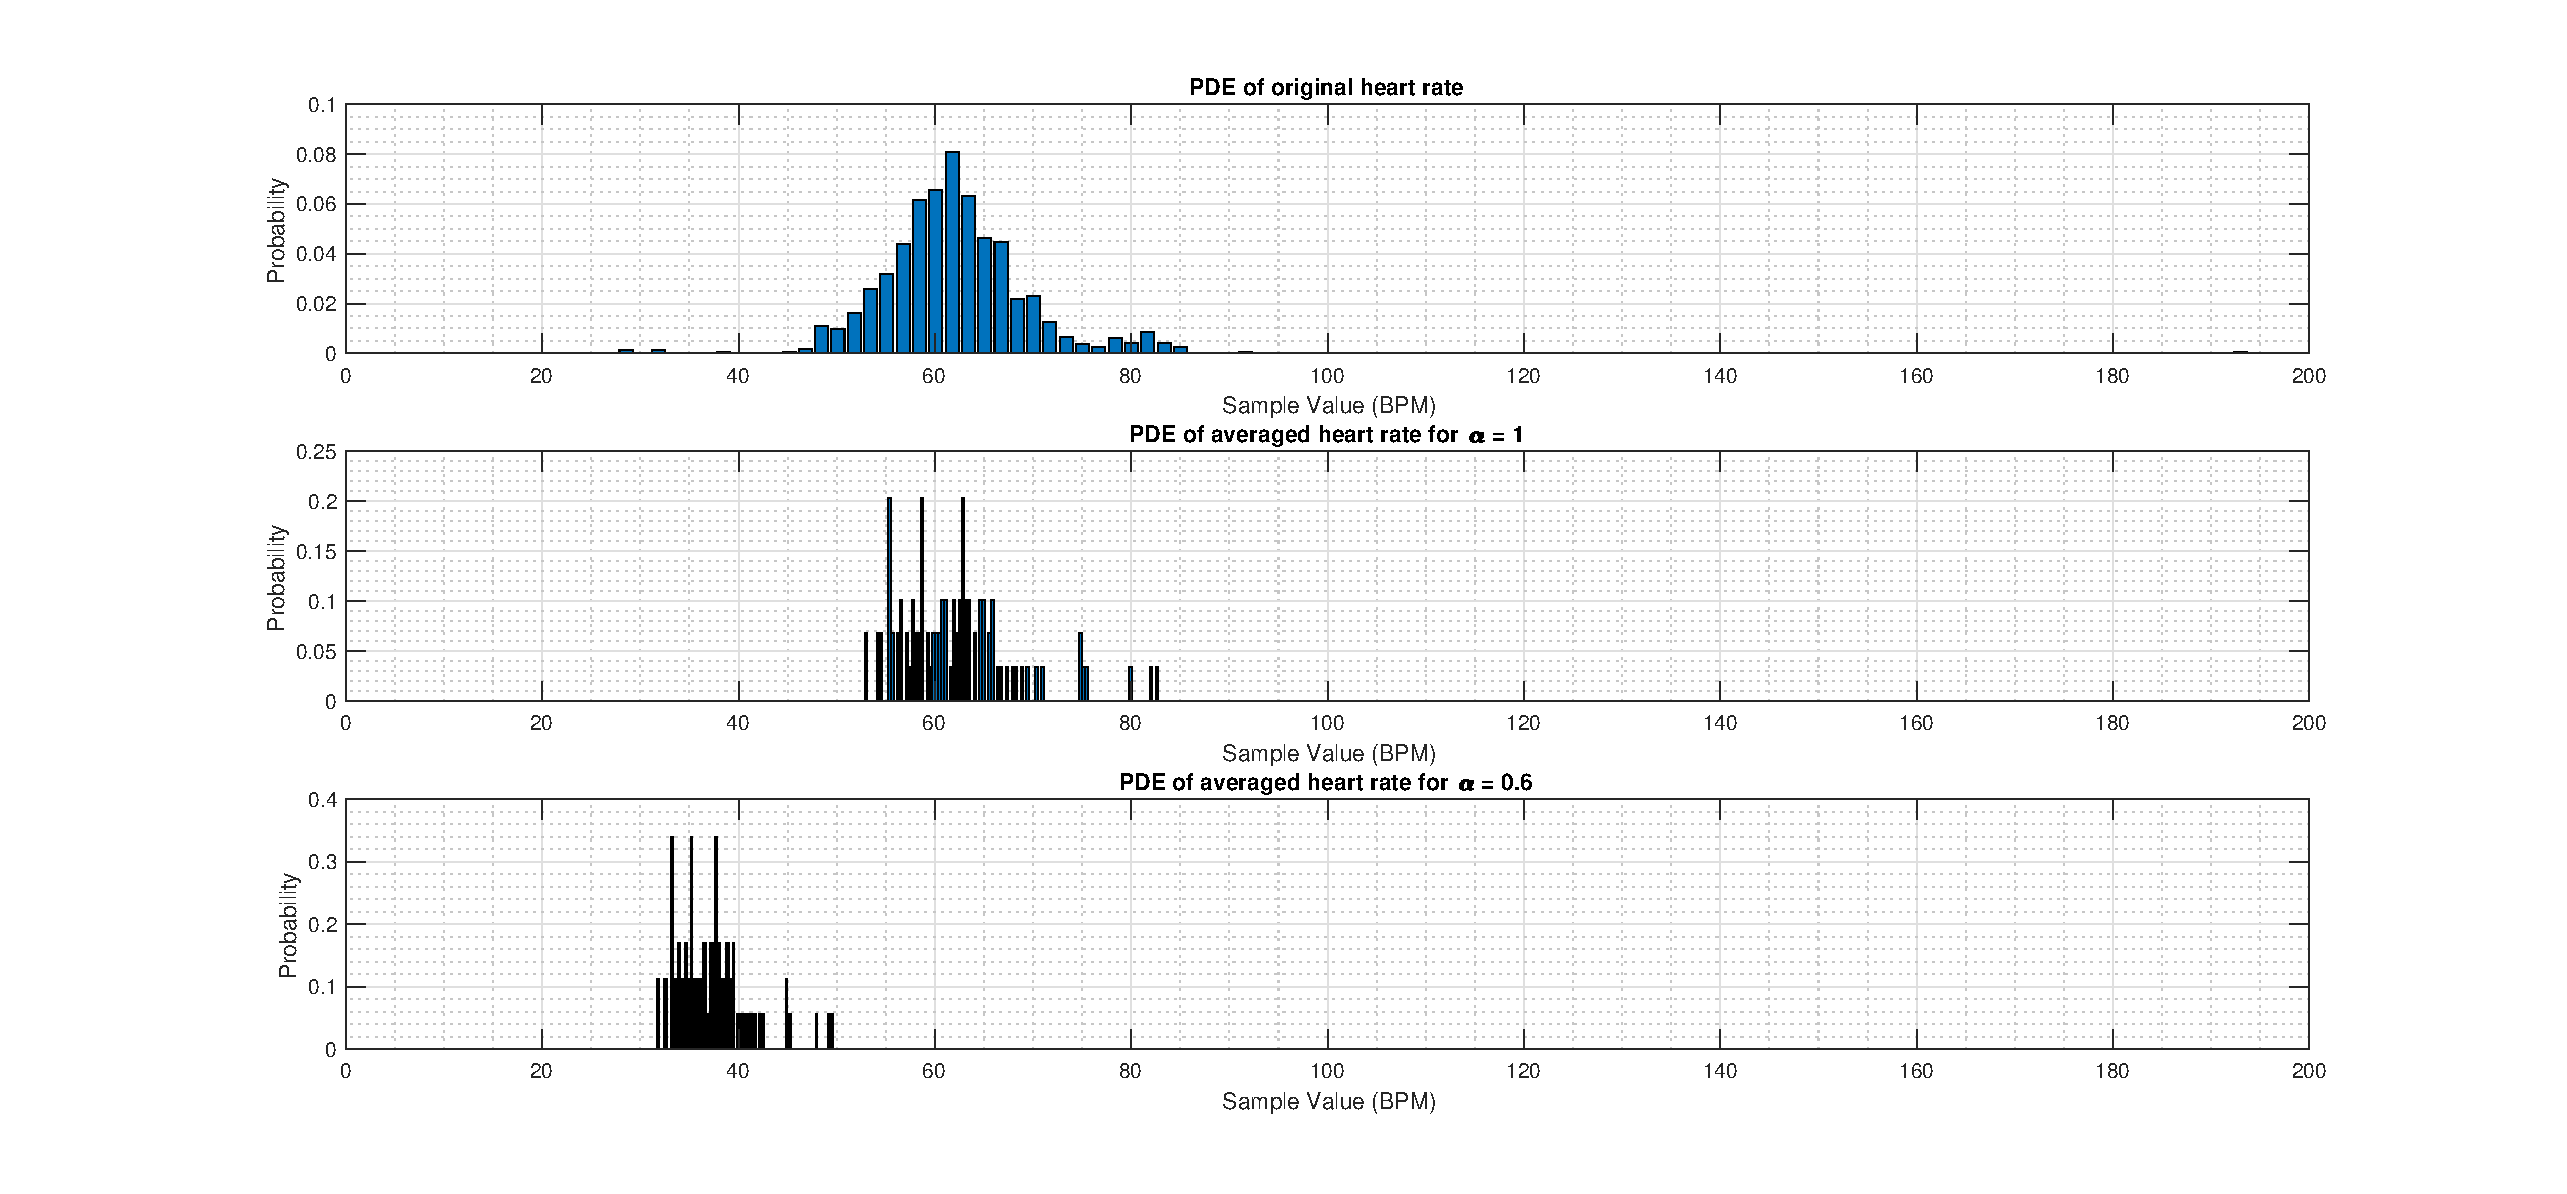
\includegraphics[width = \textwidth]{heartrate_avg}
\caption{Comparing the PDE of the original heart rate with that of the averaged heart rate for $\alpha=1,0.6$}
\label{fig:heartrate_avg}
\end{figure}

Since the \texttt{pdf.m} function from Part 1 cannot model processes that are not stationary, the heartbeat has been modeled as a stationary process. Averaging the data in blocks of B samples (in this case 10) will reduce the variance of the data to $\frac{\sigma}{B}$, which can be seen in Figure \ref{fig:heartrate_avg}.\\

Multiplying by $\alpha$ can be used to eliminate noise bias since it shifts the mean of the averaged heart rate $\hat{h}$. The factor of $\alpha$ also changes the variance of the data to $\alpha^2$.\\

Therefore, the mean of the $\alpha=1$ case is the same as that of the original data, but it has a lower variance. The $\alpha=0.6$ case has a lower mean and variance than $\alpha=1$ case as expected.

\subsubsection{AR Modeling of heart rate}

Figure \ref{fig:ar_heart} clearly shows that the heart rate data is autoregressive since it is sinusoidal and of infinite length. By contrast, Moving Average (MA) processes are of finite length and their order determines the rate of decay to 0 after some $\tau$. Note that the part of the ACF near $\tau=1000$ is particularly distorted due to the deliberately induced noise.

\begin{figure}[h!]
\centering
\begin{subfigure}{0.32\textwidth}
\centering
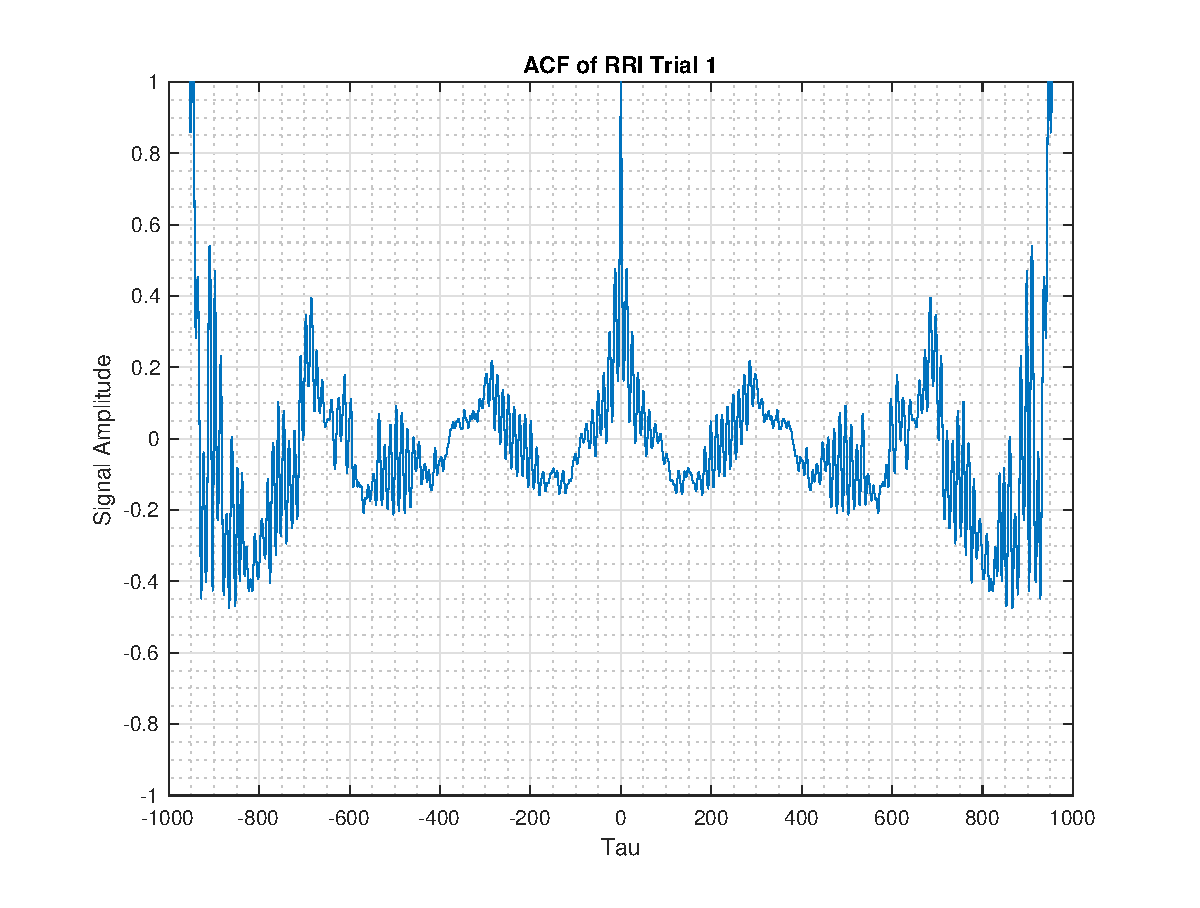
\includegraphics[width = \textwidth]{heart_acf_t1}
\caption{Trial 1}
\label{fig:heart_acf_t1}
\end{subfigure}
\begin{subfigure}{0.32\textwidth}
\centering
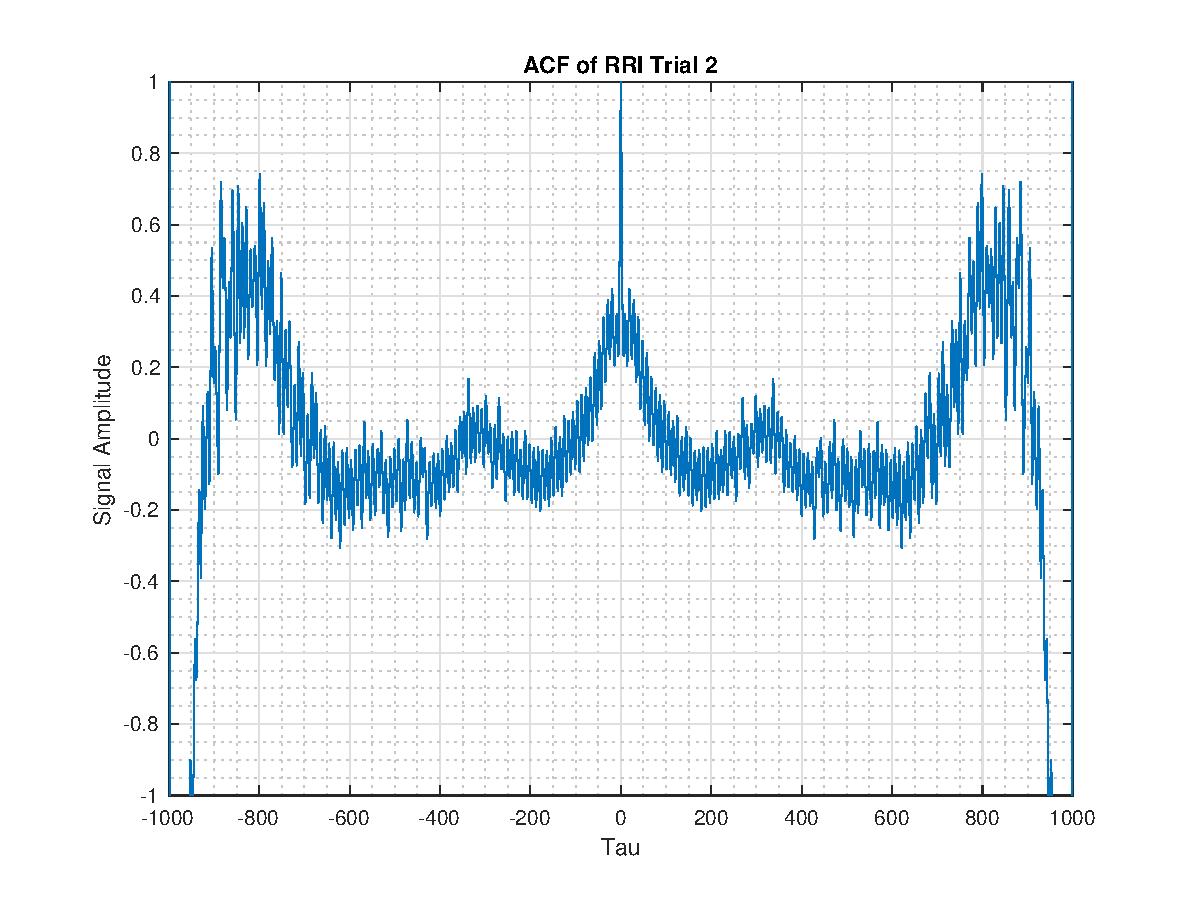
\includegraphics[width = \textwidth]{heart_acf_t2}
\caption{Trial 2}
\label{fig:heart_acf_t2}
\end{subfigure}
\begin{subfigure}{0.32\textwidth}
\centering
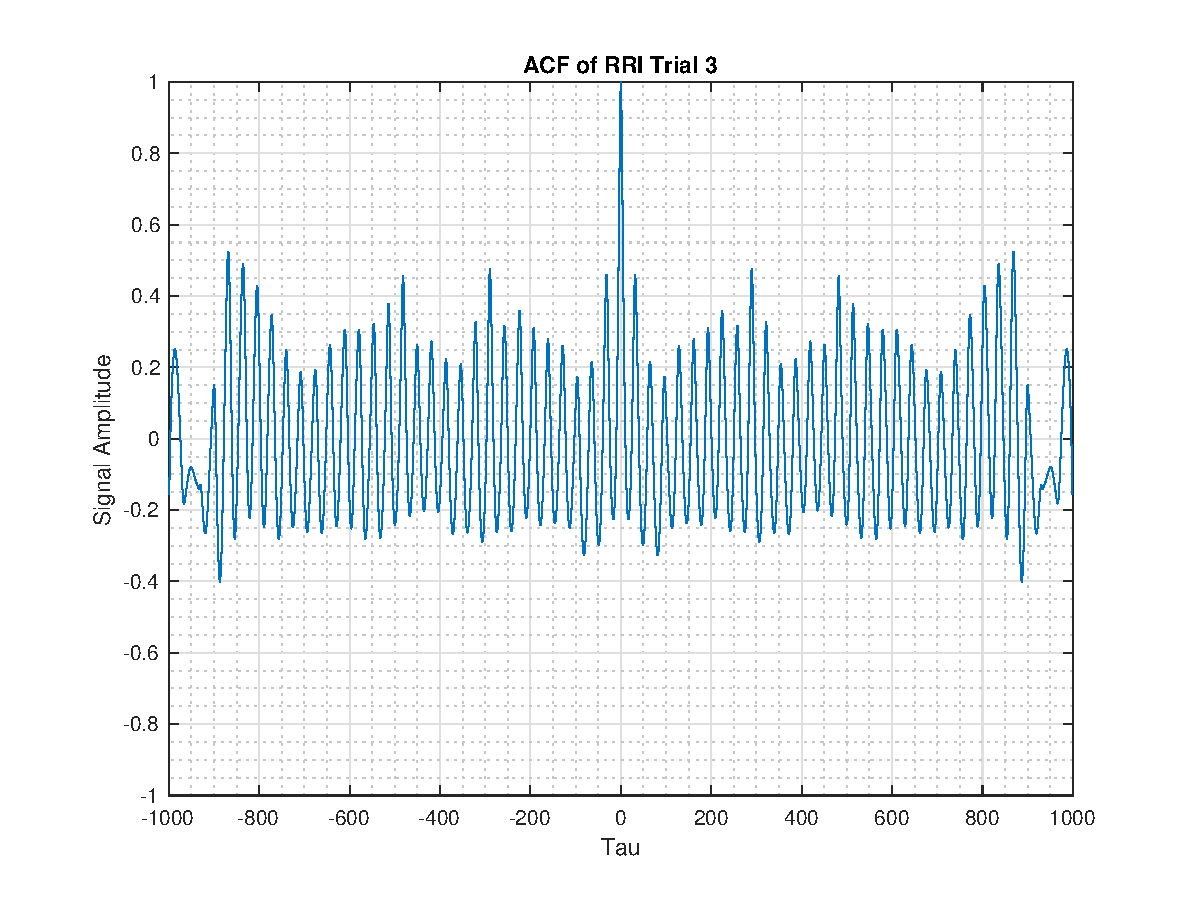
\includegraphics[width = \textwidth]{heart_acf_t3}
\caption{Trial 3}
\label{fig:heart_acf_t3}
\end{subfigure}
\caption{Autocorrelation function of RRI Trials}
\label{fig:ar_heart}
\end{figure}

Trial 1 has a global minimum for MDL at order 2, AIC at order 9, and loss function at 15. Since the PCF of trial 1 is bounded and decreasing after order 2, this process can be modeled as an AR(2) system. This is also supported by the $AIC_c$ measure.\\

\begin{figure}[h!]
\centering
\begin{subfigure}{0.32\textwidth}
\centering
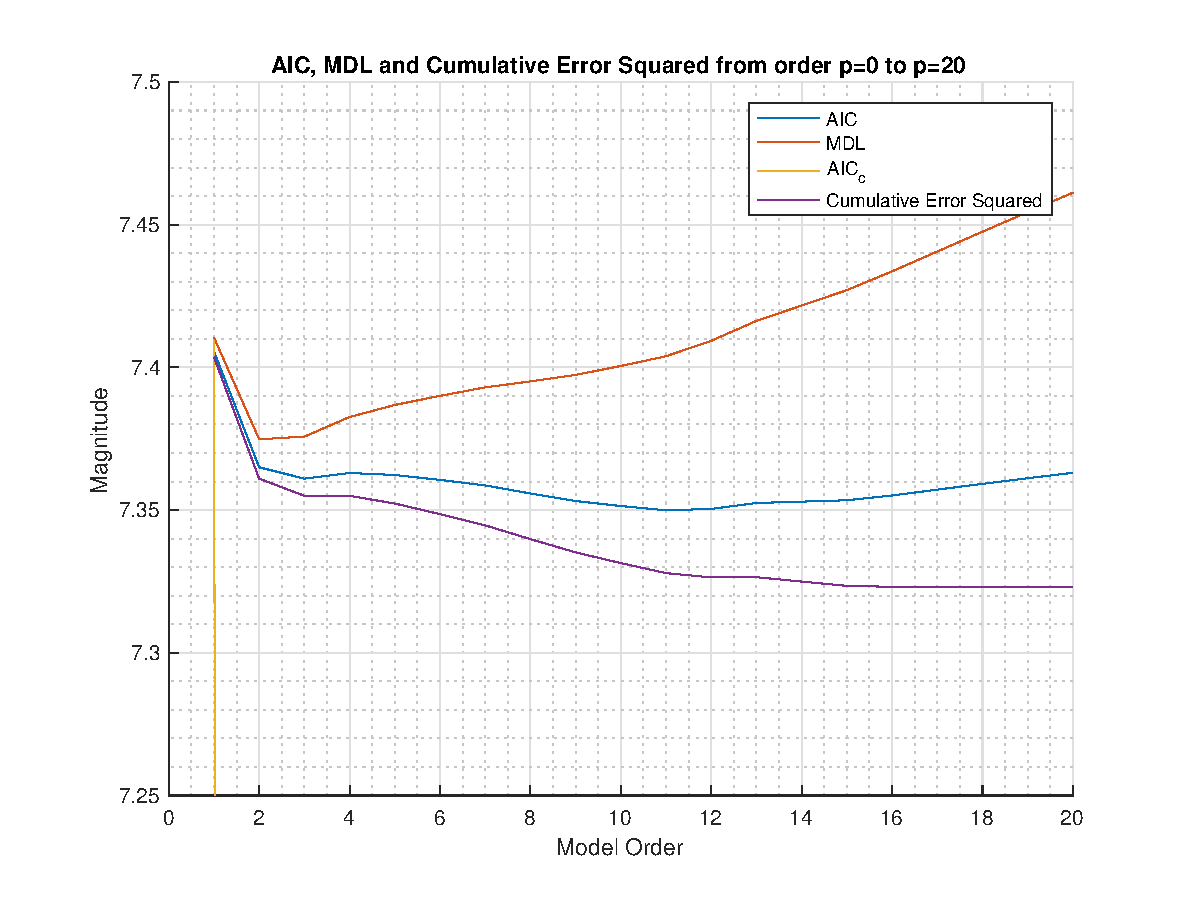
\includegraphics[width = \textwidth]{heart_mdl_t1_zoom}
\caption{MDL, AIC and Loss function}
\label{fig:heart_mdl_t1_zoom}
\end{subfigure}
\begin{subfigure}{0.32\textwidth}
\centering
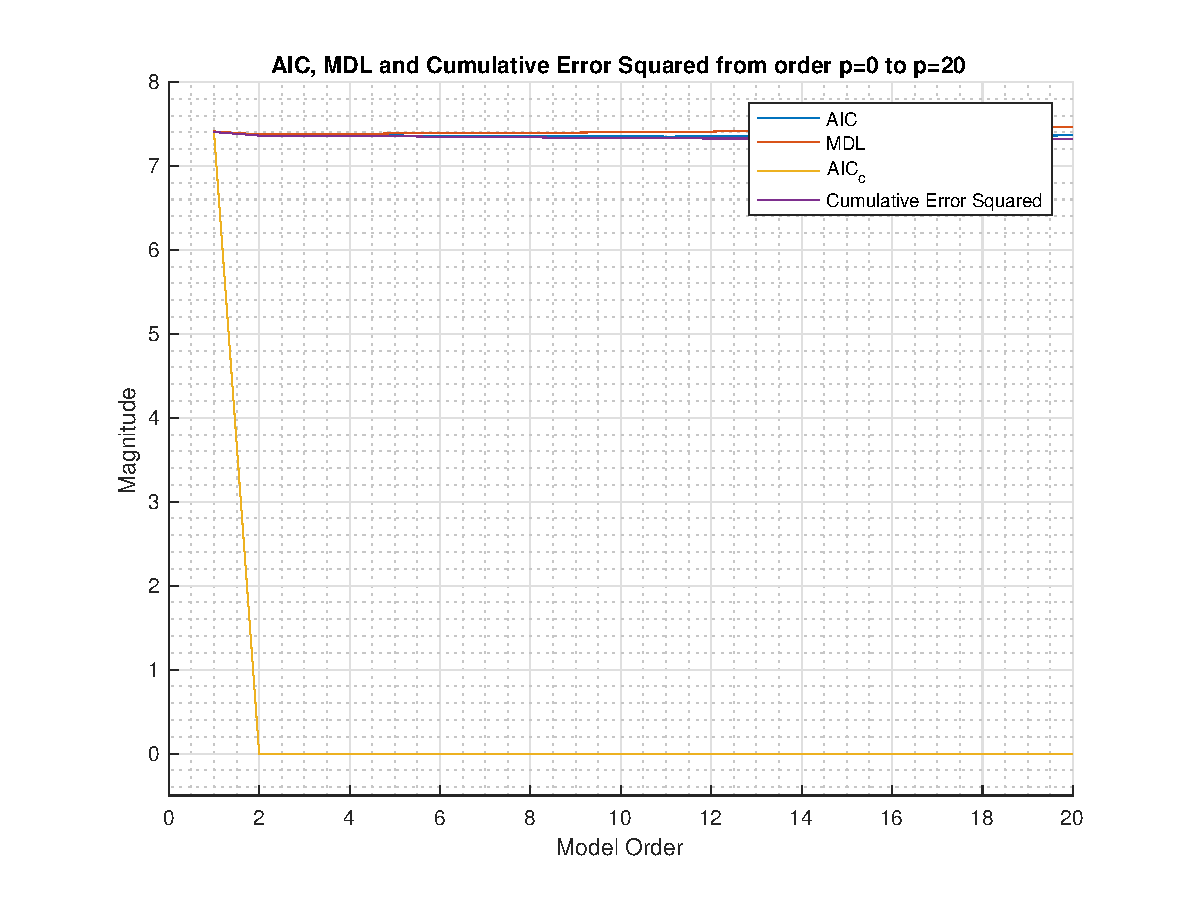
\includegraphics[width = \textwidth]{heart_mdl_t1}
\caption{Zooming out for $AIC_c$}
\label{fig:heart_mdl_t1}
\end{subfigure}
\begin{subfigure}{0.32\textwidth}
\centering
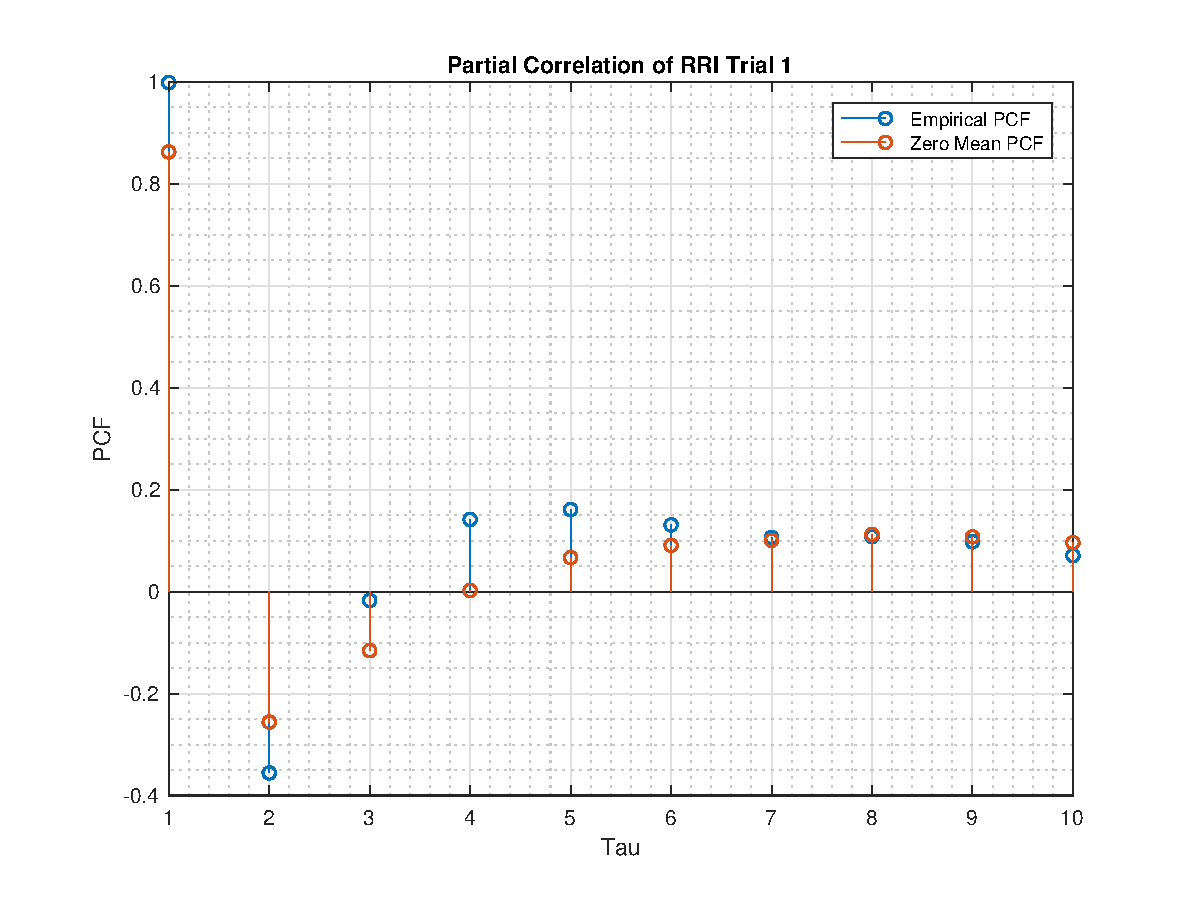
\includegraphics[width = \textwidth]{heart_pcf_t1}
\caption{Partial correlation function}
\label{fig:heart_pcf_t1}
\end{subfigure}
\caption{Model selection criteria and partial correlation function for RRI trial 1}
\label{heart_t1}
\end{figure}


Trial 2 has a global minimum for MDL at order 2, AIC at order 6, and loss function at 16. Since the PCF of trial 2 is bounded and decreasing after order 2, this process can also be modeled as an AR(2) system. Again, this is supported by the $AIC_c$ measure.\\


\begin{figure}[h!]
\centering
\begin{subfigure}{0.32\textwidth}
\centering
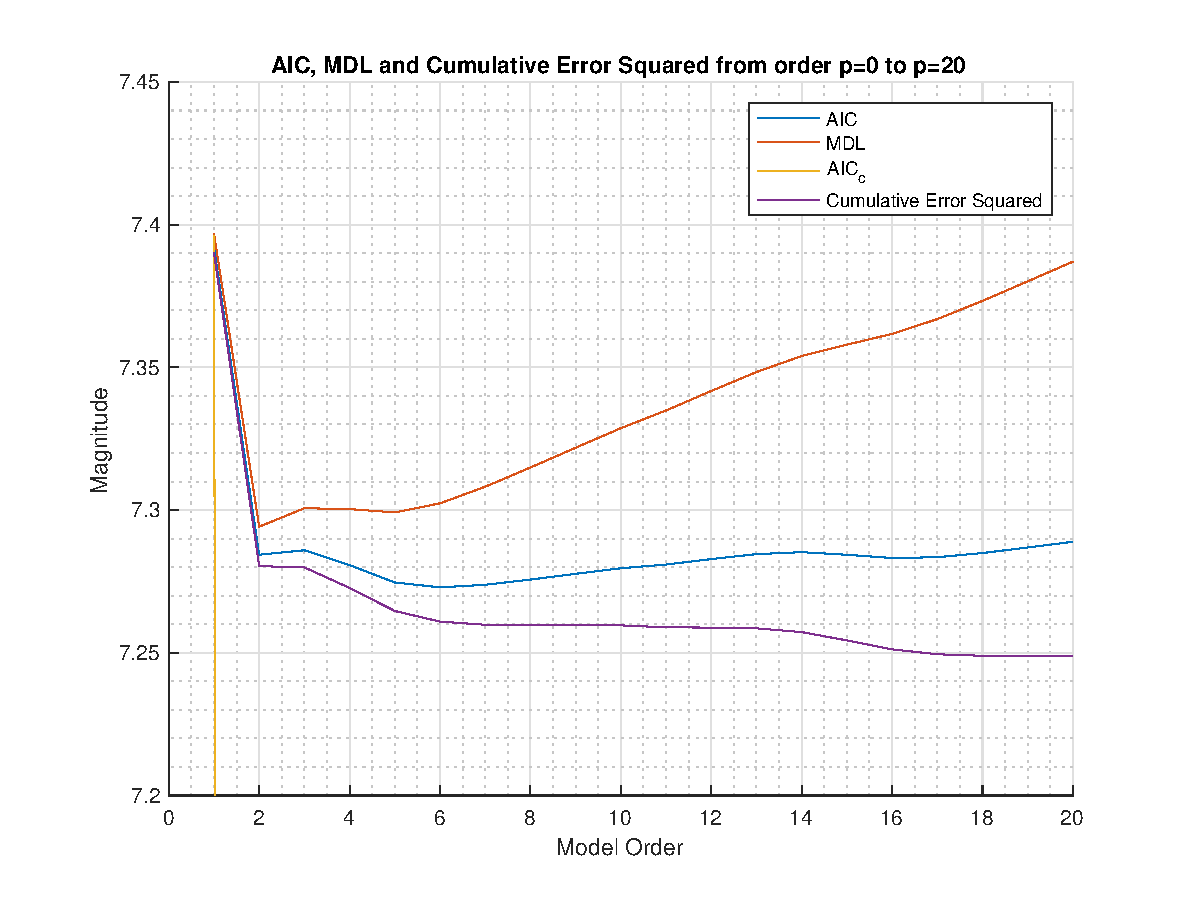
\includegraphics[width = \textwidth]{heart_mdl_t2_zoom}
\caption{MDL, AIC and Loss function}
\label{fig:heart_mdl_t2_zoom}
\end{subfigure}
\begin{subfigure}{0.32\textwidth}
\centering
\includegraphics[width = \textwidth]{heart_mdl_t2}
\caption{Zooming out for $AIC_c$}
\label{fig:heart_mdl_t2}
\end{subfigure}
\begin{subfigure}{0.32\textwidth}
\centering
\includegraphics[width = \textwidth]{heart_pcf_t2}
\caption{Partial correlation function}
\label{fig:heart_pcf_t1}
\end{subfigure}
\caption{Model selection criteria and partial correlation function for RRI trial 2}
\label{heart_t2}
\end{figure}

Trial 3 has a global minimum for MDL at order 4, AIC at order 4, and loss function at 6. However, the $AIC_c$ measure has a global minimum at order 2. Since the PCF of trial 1 is bounded and decreasing after order 2, this process can be modeled as an AR(2) system.\\

\begin{figure}[h!]
\centering
\begin{subfigure}{0.32\textwidth}
\centering
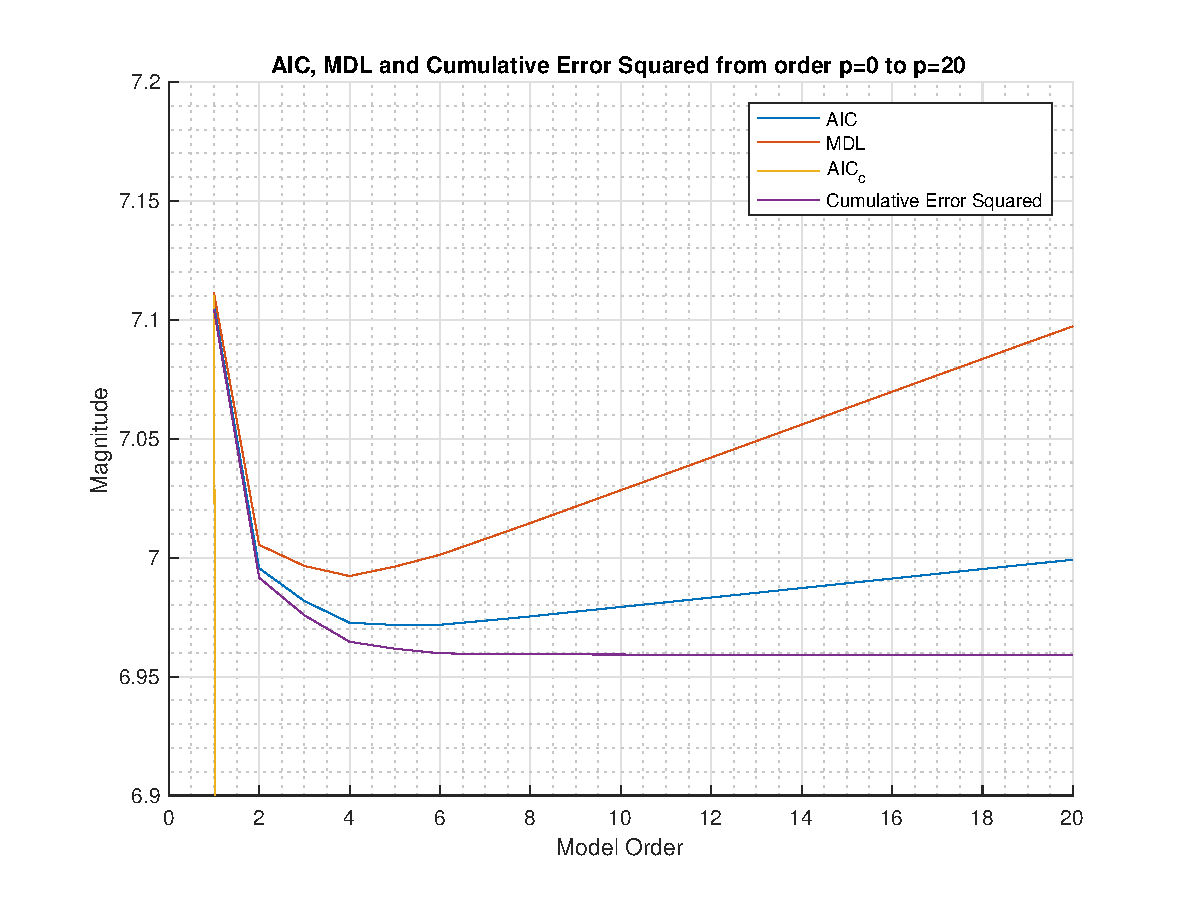
\includegraphics[width = \textwidth]{heart_mdl_t3_zoom}
\caption{MDL, AIC and Loss function}
\label{fig:heart_mdl_t3_zoom}
\end{subfigure}
\begin{subfigure}{0.32\textwidth}
\centering
\includegraphics[width = \textwidth]{heart_mdl_t3}
\caption{Zooming out for $AIC_c$}
\label{fig:heart_mdl_t3}
\end{subfigure}
\begin{subfigure}{0.32\textwidth}
\centering
\includegraphics[width = \textwidth]{heart_pcf_t3}
\caption{Partial correlation function}
\label{fig:heart_pcf_t3}
\end{subfigure}
\caption{Model selection criteria and partial correlation function for RRI trial 3}
\label{heart_t3}
\end{figure}

Thus a second order AR process is best suited to model the measured heart rate data. The PCF stays bounded after this point and the drop in the loss function is negligible for higher orders.

\end{document}
